\documentclass{book}
\usepackage{html,graphics,color}
\usepackage{graphics,color}
\title{Minsky Simulation Engine}
\bodytext{bgcolor="white"}
\pagecolor[gray]{1}
\author{}

%begin{latexonly}
%\renewcommand{\htmladdimg}[1]{\resizebox{\textwidth}{!}{\includegraphics{images/#1}}}
\renewcommand{\htmladdimg}[1]{\includegraphics{images/#1}}
\newcommand{\fwhtmladdimg}[1]{
  \noindent\resizebox{\textwidth}{!}{\htmladdimg{#1}}
}
\newcommand{\smhtmladdimg}[1]{
  \resizebox{!}{3ex}{\htmladdimg{#1}}
}
% redefine \htmlref in LaTeX mode to quote the section number
\renewcommand{\htmlref}[2]{#1 \S(\ref{#2})}
%end{latexonly}

\begin{htmlonly}
\newcommand{\fwhtmladdimg}[1]{\htmladdimg{#1}}
\newcommand{\smhtmladdimg}[1]{\htmladdimg{#1}}
\end{htmlonly}

\newcommand{\buttonIcon}[1]{
  \resizebox{!}{2ex}{\includegraphics{images/#1}}
  }

  \begin{document}
  \author{Version 3.6.0-beta.1}

  \maketitle
See also \htmladdnormallink{Modelling with Minsky}{https://sourceforge.net/projects/minsky/files/ModellingWithMinsky.pdf}.
\chapter{Introduction}
\label{Introduction}

\section{New to system dynamics?}
\label{intro:new}

Minsky is one of a family of ``system dynamics'' computer
programs. These programs allow a dynamic model to be constructed, not
by writing mathematical equations or numerous lines of computer code,
but by laying out a model of a system in a block diagram, which can then
simulate the system. These programs are now the main tool used by
engineers to design complex products, ranging from small electrical
components right up to passenger jets.


Minsky adds another means to create the dynamic equations that are
needed to define monetary flows---the ``Godley Table''---which is
discussed in the next section for users who are experienced in
system dynamics. In this section, we'll give you a quick overview of
the generic system dynamics approach to building a model.


Though they differ in appearance, they all work the same way:
variables in a set of equations are linked by wires to mathematical
operators. What would otherwise be a long list of equations is
converted into a block diagram, and the block diagram makes the causal chain
in the equations explicit and visually obvious.

For example, say you wanted to define the rate of employment as
depending on output (GDP), labor productivity and population. Then you
could define a set of equations in a suitable program (like Mathcad):

\begin{eqnarray*}
\mathrm{GDP}&:=&100\\
\mathrm{LaborProductivity}&:=&1\\
\mathrm{Population}&:=&100\\
\mathrm{Workers}&:=&\mathrm{GDP}\div\mathrm{LaborProductivity}\\
\mathrm{EmpRate}&:=&\mathrm{Workers}\div\mathrm{Population}\\
\mathrm{EmpRate}&=&1
\end{eqnarray*}

Or you could define it using a block diagram, such as Minsky:

\begin{center}
%\fwhtmladdimg{NewItem1.png}
\resizebox{\textwidth}{!}{\includegraphics{images/NewItem1.eps}}
\end{center}

For a simple algebraic equation like this, modern computer algebra
programs like Mathcad are just as good as a block diagram programs like
Vissim or Minsky. But the visual metaphor excels when you want to describe a
complex causal chain.


These causal chains always involve a relationship between stocks and
flows. Economists normally model stocks and flows by adding an
increment to a stock. For example, the level of capital $K$ is defined as
a difference equation, where capital in year $t$ is shown as being 
capital in year $t-1$ plus the investment that took place that year:

\begin{displaymath}
K_t=K_{t-1}+I_{t-1}
\end{displaymath}

The problem with this approach is that in reality, capital is
accumulating on a daily, or even hourly, basis. It is better to model
stock as continuous quantities and for this reason, all stocks and
flows in Minsky are handled instead as integral equations. The amount
of capital at time $t$ is shown as the integral of net investment
between time 0 and today:

\begin{displaymath}
K(t)=\int_0^t I(s)ds
\end{displaymath}

However, rather than being shown as an equation, the relationship is shown as a diagram:

\begin{center}
\includegraphics{images/NewItem7.eps}
\end{center}

The advantages of the block diagram representation of dynamic equations
over a list of equations are:
\begin{itemize}
\item    They make the causal relationships in a complex model
  obvious. It takes a specialized mind to be able to see the causal
  relations in a large set of mathematical equations; the same
  equations laid out as diagrams can be read by anyone who can read
  a stock and flow diagram---and that's most of us;
\item The block diagram paradigm makes it possible to store components of
  a complex block diagram in a group. For example, the fuel delivery
  system in a car can be treated as one group, the engine as another,
  the exhaust as yet another. This reduces visual complexity and also
  makes it possible for different components of a complex model to be
  designed by different groups and then ``wired together'' at a later
  stage.
\end{itemize}

For example, here's a model of a 4 cylinder engine car---one of the
simple examples distributed with the program Vissim:

\begin{center}
\fwhtmladdimg{NewItem8.png}
\end{center}

Programs like Vissim and Simulink have been in existence for almost 2
decades, and they are now mature products that provide everything
their user-base of engineers want for modeling and analyzing complex
dynamic systems. \htmlref{So why has Minsky been
  developed?}{intro:experienced}

\section{Experienced in system dynamics?}
\label{intro:experienced}

As an experienced system dynamics user (or if you've just read \htmlref{``New to
system dynamics?''}{intro:new}), what you need to know is what Minsky
provides that other system dynamics programs don't. That boils down to
one feature: The Godley Table. It enables a dynamic model of
financial flows to be derived from a table that is very similar to the
accountant's double-entry bookkeeping table.


The dynamics in financial flows could be modeled using the block diagram
paradigm. But it would also be very, very easy to make a mistake
modeling financial flows in such a system, for one simple reason:
every financial flow needs to be entered at least twice in a
system---once as a source, and once as a sink.


For example, if you go shopping and buy a new computer with your
credit card, you increase your debt to a bank and simultaneously
increase the deposit account of the retailer from whom you buy the
computer. The two system states in this model---your credit card
(``BuyerCredit'') and the retailer's deposit account
(``SellerDeposit'')---therefore have to have the same entry (let's call
this ``Card'') made into them. Such a transaction would look
like this:


\begin{center}
\includegraphics{images/NewItem11.eps}
\end{center}

That would work, but there's nothing in the program that warns you if
you make a mistake like, for example, wiring up the BuyerCredit entry,
but forgetting the SellerDeposit one:

\begin{center}
\includegraphics{images/NewItem12.eps}
\end{center}

Or, perhaps, wiring up both blocks, but giving one the wrong sign:

\begin{center}
\includegraphics{images/NewItem51.eps}
\end{center}

In a very complex model, you might make a mistake like one of the above, run the simulation and get nonsense results, and yet be unable to locate your mistake.


Minsky avoids this problem by using the paradigm that accountants
developed half a millennium ago to keep financial accounts accurately:
double-entry bookkeeping. Here is the same model in Minsky:

\begin{center}
\begin{tabular}{|c|cc|c|}
\hline
Flows $\downarrow$ / Stock Variables
$\rightarrow$&\multicolumn{1}{|c|}{$BuyerCredit$}&\multicolumn{1}{|c|}{$SellerDeposit$}&Row Sum\\\cline{2-3}&\multicolumn{1}{|c|}{asset}&\multicolumn{1}{|c|}{liability}&\\\hline
Initial Conditions&$0$&$0$&0\\
Buyer Accesses Credit&$Card$&$Card$&0\\
\hline
\end{tabular}
\end{center}

This is an inherently better way to generate a dynamic model of financial flows, for at least two reasons:
\begin{itemize}
\item All financial transactions are flows between entities. The
  tabular layout captures this in a very natural way: each row shows
  where a flow originates, and where it ends up
\item The program adopts the accounting practice of double-entry
  bookkeeping, in which entries on each row balance to zero according
  to the {\em accounting equation} (Assets=Liabilities+Equities). The source is
  shown as a positive value increasing the value of assets, the sink
  is a positive value increasing a corresponding liability. If you
  don't ensure that each flow starts somewhere and ends
  somewhere---say you make the same mistake as in the block diagram
  examples above, then the program will identify your mistake.
\end{itemize}

If you forget to enter the recipient in this transaction, then the Row
Sum identifies your mistake by showing that the row sums to ``Card''
rather than zero:

\begin{center}
\begin{tabular}{|c|cc|c|}
\hline
Flows $\downarrow$ / Stock Variables
$\rightarrow$&\multicolumn{1}{|c|}{$BuyerCredit$}&\multicolumn{1}{|c|}{$SellerDeposit$}&Row Sum\\\cline{2-3}&\multicolumn{1}{|c|}{asset}&\multicolumn{1}{|c|}{liability}&\\\hline
Initial Conditions&$0$&$0$&0\\
Buyer Accesses Credit&$Card$&&$Card$\\
\hline
\end{tabular}
\end{center}

And it also identifies if you give the wrong sign to one entry:

\begin{center}
\begin{tabular}{|c|cc|c|}
\hline
Flows $\downarrow$ / Stock Variables
$\rightarrow$&\multicolumn{1}{|c|}{$BuyerCredit$}&\multicolumn{1}{|c|}{$SellerDeposit$}&Row Sum\\\cline{2-3}&\multicolumn{1}{|c|}{asset}&\multicolumn{1}{|c|}{liability}&\\\hline
Initial Conditions&$0$&$0$&0\\
Buyer Accesses Credit&$Card$&$-Card$&$2Card$\\
\hline
\end{tabular}
\end{center}

Minsky thus adds an element to the system dynamics toolkit which is
fundamental for modeling the monetary flows that are an intrinsic
aspect of a market economy. Future releases will dramatically extend
this capability. 


\chapter{Getting Started with Minsky}
\label{Getting-Started-Minsky}
\section{System requirements}

Minsky is an open source program available for Windows, Mac OS X,
and various Linux distributions, as well as compilable on any suitable
Posix compliant system. Go to our \htmladdnormallink{SourceForge
page}{https://minsky.sourceforge.io} to download the version you need. Linux
packages are available from the \htmladdnormallink{OpenSUSE
build service}{https://build.opensuse.org/package/show/home:hpcoder1/minsky}.

\section{Getting help}

Press the F1 key, or select ``help'' from the context menu. Help is
context-sensitive.


\section{Components of the Program}

There are 6 components to the Minsky interface:

\begin{enumerate}
\item  The menus.

  \begin{tabular}{llllll}
    File & Edit & Insert & Options & Runge Kutta & Help \\
  \end{tabular}

\item  The Run buttons

\htmladdimg{NewItem15.png}

\item The simulation speed slider

\htmladdimg{NewItem16.png}

\item The Zoom buttons

\htmladdimg{NewItem17.png}

\item The Wiring and Equation tabs

\htmladdimg{WiringEquationsTab.png}

\item The design icons

\fwhtmladdimg{NewItem18.png}

\item And finally the Design Canvas--the large drawing area beneath the buttons and icons.

\fwhtmladdimg{NewItem19.png}
\end{enumerate}

\subsection{Menu}
\label{Menu}

  \begin{tabular}{llllll}
    File & Edit & Insert & Options & Runge Kutta & Help \\
  \end{tabular}

The menu controls the basic functions of saving and loading files,
default settings for the program, etc. These will alter as the program
is developed; the current menu items are: 

\subsubsection{File}
\label{File}

\begin{description}
\item[About Minsky] Tells you the version of Minsky that you are using.

\item[New System] Clear the design canvas.

\item[Open] Open an existing Minsky file (Minsky files have the suffix of ``mky").

\item[Recent Files]\label{recentfiles} Provides a shortcut to some of
your previously opened Minsky files.

\item[Library] Opens a repository of models for the Minsky simulation system.

\item[Save] Save the current file.

\item[Save As] Save the current file under a new name.

\item[Insert File as Group] Insert a Minsky file directly into the
current model as a \htmlref{group}{Group}

\item[Export Canvas] Export the current canvas into *svg, *pdf, *eps, *tex, or *m format.
  If using LaTeX (*tex), produce the set of equations that define the
  current system for use in documenting the model, for use in LaTeX
  compatible typesetting systems. If your LaTeX implemention doesn't
  support breqn, untick the \htmlref{wrap long equations
  option}{wrap-equations}, which can be found in the preferences panel under the options menu.
  If using a MatLab function this can be used to simulate the system in a MatLab compatible system,
  such as \htmladdnormallinkfoot{MatLab}{https://en.wikipedia.org/wiki/MATLAB} or 
  \htmladdnormallinkfoot{Octave}{http://www.gnu.org/software/octave/}.

\item[Log simulation] Outputs the results of the integration variables
into a CSV data file for later use in spreadsheets or plotting
applications.

\item[Recording] Record the states of a model as it is being built for later
replay. This is useful for demonstrating how to build a model, but
bear in mind that recorded logs are not, in general, portable between
versions of Minsky.

\item[Replay recording] Replay a recording of model states.

\item[Quit] Exit the program. Minsky will check to see whether you have saved your changes. If you have, you will exit the program; if not, you will get a reminder to save your changes.

\item[Debugging use] Items under the line are intended for developer
  use, and will not be documented here. Redraw may be useful if the
  screen gets messed up because of a bug.

\end{description}

\subsubsection{Edit}
\label{Edit}

\begin{itemize}
\item\label{edit:undo} Undo and Redo allow you to step back and forward in your editing
history. If you step back a few steps, and then edit the model, all
subsequent model states will be erased from the history.

\item\label{edit:copy} Cut/copy/paste. Selecting, or lassoing a region
of the canvas will select a group of icons, which will be shaded to
indicate the selected items. Wires joining two selected items will
also be selected. Note that, compatible with X-windows, selecting
automatically performs a copy, so the copy operation is strictly
redundant, but provided for users familiar with systems where an
explicit copy request is required. Cut deletes the selected
items. Paste will paste the items in the clipboard as a
\htmlref{group}{Group} into the current model. At the time of writing,
copy-pasting between different instances of Minsky, or into other
applications, may not work on certain systems. Pasting the clipboard
into a text-based application will be a Minsky schema XML document.

%begin{latexonly}
\begin{tabular}{ccc}
\resizebox{0.45\textwidth}{!}{\includegraphics{images/selectionExamplePrior.eps}} & 
\raisebox{1.5cm}{$\Rightarrow$} &
\resizebox{0.45\textwidth}{!}{\includegraphics{images/selectionExamplePost.eps}}\\
\end{tabular}
%end{latexonly}
\begin{rawhtml}
<table>
<tr>
<td><img src="selectionExamplePrior.png"></td>
<td><big>&#x21d2;</big></td>
<td><img src="selectionExamplePost.png"></td>
</tr>
</table>
\end{rawhtml}

\item\label{edit:group} Create a \htmlref{group}{Group} using the
contents of the selection. Groups allow you to organise more
complicated systems specification into higher level modules that make
the overall system more comprehensible.

\end{itemize}

\subsubsection{Insert}
\label{Insert}

This menu contains a set of \htmlref{mathematical operator
blocks}{Operations} for placement on the Canvas. You can get the same
effect by clicking on the Design Icons. Also present are entries for
\htmlref{Godley table items}{godley} and \htmlref{Plots}{PlotWidget}.


\subsubsection{Options}
\label{Options}

The options menu allows you to customise aspects of Minsky.

\begin{description}
\item[Preferences]\mbox{}

\begin{itemize}
\item Godley table show values. When ticked, the values of flow
variables are displayed in the Godley table whilst a simulation is
running. This will tend to slow down the simulation somewhat.
\item Godley table output style --- whether $+/-$ or DR/CR (debit/credit)
  indicators are used.
\item Enable multiple equity columns - whether Godley table have more
  than one equity columns.
\item Number of recent files to display --- affects the \htmlref{recent
files}{recentfiles} menu.
\item\label{wrap-equations} Wrap long equations in LaTeX export. If ticked, use the breqn
package to produce nicer looking automatically line-wrapped
formulae. Because not all LaTeX implementations are guaranteed to
support breqn, untick this option if you find difficulty.
\item\label{font} select a font for variable names etc.
\end{itemize}

\item[Background colour] --- select a colour from which a colour scheme
is computed.

\end{description}

\subsubsection{Simulation}
\label{RungeKutta}

\begin{itemize}
\item Time unit allows one to specify units for the time dimension for
  dimensional analysis. eg ``year'', ``s'' etc.
\item Controls aspect of the adaptive Runge-Kutta equation solver, which
trade off performance and accuracy of the model. 
\item Note a first order explicit solver is the classic Jacobi method, which is the fastest,
but least accurate solver. 
\item The algorithm is adaptive, so the
step size will vary according to how stiff the system of equations
is. 
\item Specifying a minimum step size prevents the system from stalling,
at the expense of accuracy when the step size reaches that
minimum. 
\item Specifying a maximum step size is useful to ensure one has
sufficient data points for smooth plots.
\item An iteration is the time between updates to plots, increasing the
number of solver steps per iteration decreases the overhead involved
in updating the display, at the expense of smoothness of the
plots. Screen refresh is the period between screen updates, in ms. If
an iteration takes less than this time, the screen refresh is postponed
until the time has expired. 100ms is fast enough for a smooth
animation of the simulation - increasing this value will improve
simulation performance at the cost of a jerky animation of the
simulation.
\item Start time is the value of the system $t$ variable when the
  system is reset.
\item Run until time can be used to pause the simulation ince t
  reaches a certain value. Setting this to ``Infinity'' causes the
  simulation to run indefinitely, or until some arithmetic error
  occurs.
\end{itemize}

\subsubsection{Help}
\label{Help}

Provides an in-program link to this manual. Note that pressing F1 will
also launch help windows in a cintext sensitive way, ie it will open
the relevant help section for where ever the mouse is over. Similarly,
each item on the canvas has a help menu item in the context menu
relevant for that item.

\subsection{Record/Replay Buttons}
\label{RecReplayButtons}

\htmladdimg{recReplayButtons.png}

These buttons control the recording / replay mode of Minsky. You can
record your interactions with Minsky, and replay those interactions
for demonstration/presentation purposes. 

\begin{enumerate}
  \item Record a session of building/modifying a model. Note that
    replaying a recorded session always starts from a blank canvas, so
    if you're recording the modification of a model, ensure that the
    first thing recorded is to load the model being modified. This
    button is a toggle button, so clicking it again finishes the
    session, and closes the file.
  \item Simulate/Replay button. Pressing this button changes Minsky
    into replay mode, and asks for a recording file. You may use the
    run buttons (run/pause,stop and step), as well as the speed
    slider, to control the replay. This button is a toggle button, so
    clicking it again returns Minsky back to the default simulation
    mode.
\end{enumerate}

\subsection{Recalculate button}
\label {Recalculate}

\htmladdimg{recalculate.png}

The recalculate button computes the values of all variables at the
start of simulation. It is particularly useful for recalculating the
state of the model with tensor valued data.

\subsection{Run Buttons}
\label{RunButtons}

\htmladdimg{NewItem15.png}

The Run buttons respectively:
\begin{enumerate}
\item    Start a simulation--when started the button changes to a pause icon,
allowing you to pause the simulation \htmladdimg{NewItem23.png}.
\item Stop a simulation and reset the simulation time to zero
\item Step through the simulation one iteration at a time.
\item Reverse checkbox changes the simulation time direction. Bear in
  mind that a simulation will eventually diverge from its original
  trajectory due to chaotic effects.
\end{enumerate}

%\subsection{Manipulating items on the canvas}
%
%\begin{description}
%\item[To move] and item, click on the interior of an item and drag it
%to the new position.
%\item[To wire items] click on the small circle representing the output
%port, and drag out a wire towards an input port on another item.
%\item[To lasso], click outside of any item and drag out a rectangular
%region.
%\item[To pan] the canvas, hold the shift key down whilst dragging on
%the canvas.
%\end{description}

%\begin{description}
%\item[Wire] This draws wires that connect one operator on the Canvas
%to another. For example, if you have placed these icons on the
%Palette: 
%
%\htmladdimg{NewItem24.png}
%
%and you now want to link them together into an equation, then click on
%the Wire button, move the cursor to the right end of GDP, and click
%and drag to the top of the divide symbol:
%
%\htmladdimg{NewItem25.png}
%
%Do the same for LabProd, and to attach the Divide icon to the left
%hand side of Workers, and you've defined the equation that the number
%of workers employed equals GDP divided by labor productivity. The
%flowchart will look like this: 
%
%\htmladdimg{NewItem26.png}
%
%And this is the equation you have now created:
%\begin{displaymath}
%\mathrm{Workers}=\frac{\mathrm{GDP}}{\mathrm{LabProd}}
%\end{displaymath}
%
%\item[Move] This is the default mode for the mouse, and it lets you:
%
%\begin{itemize}
%\item Move already entered icons around the Canvas by clicking on
%them, holding the mouse button down, and releasing it when you have
%got to the desired location; 
%\item Select an item from the Design Icons and place it on the
%Canvas. When you first click on an Icon, it will either appear at the
%top left hand corner of the Canvas, or bring up a menu where you enter
%various essential details (Name, value etc.), after which the Icon
%appears at the top left hand corner of the Canvas. It will then snap
%to wherever the mouse cursor currently is, and can be placed on the
%Canvas by clicking.
%\end{itemize}
%\item[Pan] This moves all the Icons on the Canvas as a group, which is useful
%when you have a very large model and you want to move to a small part
%of it. Choose Pan, click and hold the mouse button down, and then move
%the mouse. The entire model will shift with the mouse.
%
%\item[Lasso] Lassoing is the first step in creating a Group, or
%selecting multiple Icons for some operation (copying, deleting,
%etc.---these are not yet implemented but will be in the next major
%release).
%\end{description}
%
%        Grouping. Choose Lasso, click and hold down the mouse button,
%        then drag over the region you wish to make into a group:
%
%\htmladdimg{NewItem117.png}
%
%
%Release the mouse button, and a box will be drawn around the selected
%items which can now be moved as a single entity. The inputs to the
%group are noted on the input side of the group, and the outputs on the
%output side:
%
%\htmladdimg{NewItem118.png}
%
%One unique feature of Minsky (when compared to existing system
%dynamics programs) is that the contents of the group can still be seen
%inside the group window, and they can also be edited from there. In
%the next image, the contents of the group were moved more cleanly
%inside the group (this feature is still being implemented, so some
%tidying up was needed, but was possible without having to open the
%group in a separate window):
%
%
%\htmladdimg{NewItem119.png}

\subsection{Speed slider}
\label{Speedslider}

\begin{center}
\htmladdimg{NewItem16.png}
\end{center}

The speed slider controls the rate at which a model is simulated. The
default speed is the maximum speed your system can support, but you
can slow this down to more closely observe dynamics at crucial points
in a simulation.

\subsection{Zoom buttons}
\label{ZoomButtons}

\begin{center}
\htmladdimg{NewItem17.png}
\end{center}

The Zoom buttons zoom in and out on the wiring canvas. The same functionality
is accessed via the mouse scroll wheel. The reset zoom button
\buttonIcon{zoomOrig.eps} resets the zoom level to 1, and also
recentres the canvas. It can also be used to recentre the equation
view.

The zoom to fit button zooms the model so that it just fits in the
current canvas window.

\subsection{Simulation time}
\label{SimTime}

In the right hand top corner is a textual display of the current
simulation time $t$, and the current (adaptive) difference between
iterations $\Delta t$.

\subsection{Wiring and Equations Tabs}
\label{WiringEquationsTab}

\htmladdimg{WiringEquationsTab.png}

This allows you to switch between the visual block diagram wiring view and the more 
mathematical equations view.

\subsection{Design Icons}

\fwhtmladdimg{NewItem18.png}

These are the ``nuts and bolts'' of any system dynamics program. The
number of icons will grow over time, but the key ones are implemented
now: 

\begin{description}
\item[Import data] \buttonIcon{importData.eps} Opens an import CSV file dialog, allowing the
  creation of a parameter from a CSV data file. See
  \htmlref{Importing CSV files}{Operation:csvImport}.

\item[Ravel] See \htmlref{Ravel}{Ravel}.
  
\item[Plot widget] \buttonIcon{plot.eps} Add \htmlref{plots}{PlotWidget} to the canvas.

\item[Sheet widget] \buttonIcon{sheet.eps} Add a \htmlref{sheet}{Sheet} to the canvas.

\item[Variable]  \buttonIcon{var.eps}. \label{Variable}

This is a pull down menu, giving access to creating variables,
constants and parameters.

  Variables are entities
whose value changes as a function of time and its relationship with
other entities in your model. Click on it and a variable definition
window will appear:

\begin{center}
\scalebox{0.5}{\htmladdimg{NewItem32.png}}
\end{center}

The only essential step here is providing a name for the Variable. You
can also enter a value for it (and a rotation in degrees), but these
can be omitted. In a dynamic model, the value will be generated by the
model itself, provided its input is wired.


When you click on OK (or press Enter), the newly named variable will
appear in the top left hand corner of the Canvas. Move the mouse
cursor to where you want to place the variable on the Canvas, click,
and it will be placed in that location.


Constants are entities whose
value is unaffected by the simulation or other entities in the
model. Click on it and a constant definition window will appear:

\begin{center}
\scalebox{0.5}{\htmladdimg{NewItem34.png}}
\end{center}

The only essential element here is its
value. You can also specify its rotation on the Canvas in degrees. This lets you vary a
parameter while a simulation is running---which is useful if you wish
to explore a range of policy options while a model is running.

A constant is just a type of variable, which also include parameters
(named constants), flow variables, stock variables and integration
variables. In fact there is no real conceptual difference between
creating a constant or creating a variable, as you can switch the type
using the type field.

Like the variable and constant button, the parameter button creates a
variable defaulting to the parameter type. Parameters differ from flow
variables in not having an input port, and differ from constants in
having a name and being controllable by a slider during simulation.

\item[Lock] Lock widgets are used with \htmlref{Ravels}{Ravel}.
\item[Notes] Add \htmlref{textual annotations}{Notes}

\item[Time] \buttonIcon{time.eps} embeds a reference to the
simulation time on the Canvas. This is not necessary in most
simulations, but can be useful if you want to make a time-dependent
process explicit, or control the appearance of a graph. 

For example, by default a graph displays the simulation time on the
horizontal axis, so that cycles get compressed as a simulation runs
for a substantial period:

\begin{center}
\resizebox{\textwidth}{!}{\includegraphics{images/NewItem36.eps}}
\end{center}

If a Time block is added to the marker for the x-axis range, you can
control the number of years that are displayed. This graph is set up
to show a ten year range of the model only: 

\begin{center}
\resizebox{\textwidth}{!}{\includegraphics{images/NewItem37.eps}}
\end{center}

\item[Unary functions]\buttonIcon{sqrt.eps} These are a fairly standard
complement of mathematical functions.

\item[Binary operations]
    \buttonIcon{add.eps}. These execute the stated binary
    mathematical operations. Each input can take multiple wires as
    well---so that to add five numbers together, for example you can wire 1 input
    to one port on the Add block, and the other four to the other
    port. 

Min \& Max Functions These take the minimum and maximum values, respectively.
These also allow multiple wires per input.

Pow and log. These are binary operations (taking two
arguments). In the case of the power operation, the exponent is the
top port, and the argument to be raised to that exponent is the bottom
port. This is indicated by the $x$ and $y$ labels on the ports. In the
case of logarithm, the bottom port (labelled $b$) is the base of the
logarithm.

Logical Operators $<$ $\le$, =, $\wedge$ $\vee$ $\neg$ (and,
  or, not)] These return 0 for false and 1 for true.

\item[Reduction operations]\buttonIcon{sum.eps} This menu contains
  operations that reduce a vector to a scalar, or reduce the rank of a
  tensor. Typically sum, product, any, all etc.

\item[Scans]\buttonIcon{runningSum.eps} These are running sums and the
  difference operator

\item[Miscellaneous tensor operations]\buttonIcon{outerProduct.eps}
  Any other tensor function not covered elsewhere.

\item[Switch] \buttonIcon{switchIcon.eps} Add \htmlref{a piecewise-defined function block}{SwitchIcon} 
to the canvas. Also known as a hybrid function.

\item[User defined function]\buttonIcon{userFunction.eps} You can
  define \htmlref{your own function}{Operation:userFunction} using an algebraic expression, such as \verb+exp(-x^2+y)+.

\item[Godley Table] \buttonIcon{NewItem29.eps}. \label{GodleyTable} This is the
fundamental element of Minsky that is not found (yet) in any other
system dynamics program. 

Clicking on it and placing the resulting Bank Icon on the Canvas
enters a Godley table into your model:

\begin{center}

\includegraphics{images/NewItem29.eps}
\end{center}

Double-click on the Bank Icon (or right-click and choose ``Open Godley
Table'' from the context menu) and you get a double-entry bookkeeping
table we call a Godley Table, which looks like the following onscreen:

%\fwhtmladdimg{NewItem30.png}
\begin{center}
  \scalebox{0.5}{\includegraphics{images/emptyGodley.eps}}
\end{center}

 
Use this table to enter the bank accounts and financial flows in your model. We discuss this later in the \htmlref{Tutorial (Monetary)}{tut:basicBankModel}.

\item[Integration] \buttonIcon{int.eps}.\label{Integrate}
  This inserts a variable whose value depends on the integral of other
  variables in the system. This is the essential element for defining
  a dynamic model. Click on it and the following entity will appear at
  the top left hand side of the canvas (and move with your mouse until
  you click to place it somewhere:

\begin{center}
\includegraphics{images/NewItem39.eps}
\end{center}

``int1'' is just a placeholder for the integration variable, and the
first thing you should do after creating one is give it a
name. Double-click on the ``int1'', or right click and choose
Edit. This will bring up the following menu:

\begin{center}
\scalebox{0.5}{\htmladdimg{NewItem40.png}}
\end{center}

Change the name to something appropriate, and give it an initial
value. For example, if you were building a model that included
America's population, you would enter the following:

\begin{center}
\scalebox{0.5}{\htmladdimg{NewItem41.png}}
\end{center}


The integrated variable block would now look like this:

\begin{center}
\includegraphics{images/NewItem42.eps}
\end{center}


To model population, you need to include a growth rate. According to
Wikipedia, the current US population growth rate is 0.97 percent per
annum.  Expressed as an equation, this says that the annual change in
population, divided by its current level, equals 0.0097: 

\begin{displaymath}
\frac{1}{\mathrm{Population}(t)}\cdot\left(\frac{d}{dt}\mathrm{Population}(t)\right)=0.0097
\end{displaymath}

To express this as an integral equation, firstly we multiply both
sides of this equation by Population to get:

\begin{displaymath}
\frac{d}{dt}\mathrm{Population}(t)=0.0097\cdot\mathrm{Population}(t)
\end{displaymath}

Then we integrate both sides to get an equation that estimates what
the population will be T years into the future as:

\begin{displaymath}
\mathrm{Population}(T)=315+\int_0^T 0.0097\cdot\mathrm{Population}(t)
dt
\end{displaymath}

Here, 315 (million) equals the current population of the USA, the year
zero is today, and $T$ is some number of years from today. The same
equation done as a block diagram looks like this: 

\begin{center}
\resizebox{\textwidth}{!}{\includegraphics{images/NewItem46.eps}}
\end{center}

Or you can make it look more like the mathematical equation by
right-clicking on ``Population'' and choosing ``Copy Var''. Then you will
get another copy of the Population variable, and you can wire up the
equation this way:

\begin{center}
\resizebox{\textwidth}{!}{\includegraphics{images/NewItem47.eps}}
\end{center}

Either method can be used. I prefer the latter because it's neater,
and it emphasizes the link between the simple formula for a percentage
rate of change and a differential equation. 

\item[Derivative Operator] \buttonIcon{differentiate.eps} This operator symbolically differentiates its input,
provided the input is differentiable. An error is generated if the input
is not differentiable.

\end{description}

\subsection{Design Canvas}
\label{DesignCanvas}\label{tabs:Wiring}

The Design Canvas is where you develop your model. A model consists of
a number of blocks---variables, constants and mathematical
operators---connected by wires. 

The canvas is {\em zoomable}, either via the zoom buttons on the toolbar, or
via the mouse scroll wheel. It is also {\em pannable}, either via the
scroll bars on the right and bottom, or by holding the shift key and
first mouse button together. The canvas is effectively unlimited,
however the scroll bars treat the canvas as a $10000\time10000$ pixels
in size.

\fwhtmladdimg{NewItem19.png}

\subsection{Equations tab}\label{tabs:Equations}

This displays the mathematical representation of the model

\subsection{Parameters tab}\label{tabs:Parameters}

This displays the properties of all parameters defined in the model,
in one place.

\subsection{Variables tab}\label{tabs:Variables}

This displays the properties of selected variables in the model. The
variables can be displayed on the tab by selecting ``Display variable
on tab'' in it's context menu. It may be hidden on the design canvas
if it is not required for the definition of something else. This can
be a place to keep less important variables ``out of sight''.

\subsection{Plots tab}\label{tabs:Plots}

Shows all plots in one place

\subsection{Godleys tab}\label{tabs:Godleys}

Shows all Godley tables in one place.

\subsection{Wires}
\label{Wires}

The wires in a model connect blocks together to define equations. For
example, to write an equation for 100/33, you would place a
\buttonIcon{const.eps} on the canvas, and give it the value of 100:

\begin{center}
\scalebox{0.5}{\htmladdimg{NewItem122.png}}
\end{center}

Then do the same for 33, and place a divide block on the canvas:

\begin{center}
\includegraphics{images/NewItem123.eps}
\end{center}

Then click on the right hand edge of \buttonIcon{const100.eps}
and drag to extend the wire to the numerator ($\times$) port of the divide operation.

\begin{center}
\includegraphics{images/wireExample1.eps}
\end{center}

Finally, add the other wire.
\begin{center}
\includegraphics{images/wireExample2.eps}
\end{center}

\section{Working with Minsky}

\subsection{Components in Minsky}

There are a number of types of components in Minsky
\begin{enumerate}
\item Mathematical operators such as plus (+), minus (-)
\item Constants (or parameters, which are named constants) which are
given a value by the user 
\item Variables whose values are calculated by the program during a simulation and depend on the values of constants and other variables; and
\item Godley Tables, which define both financial accounts and the
flows between them. In the language of stock and flow modelling, the
columns of a Godley table are the stocks, which are computed by
integrating over a linear combination of flow variables.
\item Integrals --- represent a variable computed by integrating a
function forward in time.
\item Groups, which allow components to be grouped into modules that
can be used to construct more complex models.
\end{enumerate}


\subsection{Inserting a model component}


There are five ways to insert a component of a model onto the Canvas:
\begin{enumerate}
\item Click on the desired Icon on the Icon Palette, drag the block
onto the Canvas and release the mouse where you want to insert it 

\begin{center}
\fwhtmladdimg{NewItem18.png}
\end{center}

\item Choose Insert from the menu and select the desired block there

  \begin{center}
    %begin{latexonly}
    \resizebox{!}{0.6\textheight}{
      %end{latexonly}
      \htmladdimg{NewItem159.png}
     %begin{latexonly}
    }
    %end{latexonly}
  \end{center}
  \newpage
  
\item Right-click on an existing block and choose copy. Then place the
copy where you want it on the palette. 

\begin{center}
\htmladdimg{NewItem161.png}
\end{center}

\item Variables can be inserted by typing the variable name on the
  canvas, and constants enetered by typing the numerical
  value. Similarly, operations can be inserted by typing the operator
  name (eg \verb+sin+, or \verb+*+). Notes can be inserted by starting
  the note with a \verb+#+ character.

\item Variables can also be picked from the \hyperref[ref]{Variable
    Browser}{Variable Browser}{}{VariableBrowser} and placed on the canvas.
\end{enumerate}


\subsection{Creating an equation}

Equations are entered in Minsky graphically. Mathematical operations
like addition, multiplication and subtraction are performed by wiring
the inputs up to the relevant mathematical block. The output of the
block is then the result of the equation. 

For example, a simple equation like
\begin{displaymath}
100/3 = 33.3
\end{displaymath}
is performed in Minsky by defining a constant block with a value of 100, defining another with a value of 3, and wiring them up to a divide-by block. Then attach the output of the divide block to a variable, and run the model by clicking on\smhtmladdimg{NewItem130.png} :

\begin{center}
  \includegraphics{images/NewItem129.eps}
\end{center}

If you click on the equation tab, you will see that it is:

\begin{displaymath}
\mathrm{Answer}=\frac{100}{3}
\end{displaymath}

Very complex equations---including dynamic elements like integral
blocks and Godley Tables---are designed by wiring up lots of
components, with the output of one being the input of the next. See
the tutorial for examples.

\subsection{Wiring components together}

A model is constructed by wiring one component to another in a way
that defines an equation. Wires are drawn from the output port of one
block to the input port of another. Ports are circles on the blocks to
which wires can be attached, which can be seen when hovering the
pointer over the block. Variables have an input and an output
port; constants and parameters only have an output port. A
mathematical operator has as many input ports as are needed to define
the operation.


To construct an equation, such as Fred - Wilma = Barney:

Click the mouse near the output port of one block and drag the
cursor to the input port of another while holding the mouse button
down. An arrow extends out from the output port. Release the mouse
button near the required input port of the operator. A connection will
be made.

\begin{center}
\includegraphics{images/NewItem181.eps} 
\end{center}


The equation is completed by wiring up the other components in the same way.

\begin{center}
\includegraphics{images/NewItem182.eps} 
\end{center}


\subsection{Creating a banking model}
\label{creatingBankingModel}

\subsubsection{Creating a bank}

The first step in creating a model with a banking sector is to click on the Godley Table Icon in the Icon Palette, and place the block somewhere on the Canvas.

\subsubsection{Entering accounts}

Double click or right click on the Godley table block to bring up the
Godley Table. The table is divided up into sections representing the
different accounting asset classes: Asset, Liability and
Equity. Assets represent what you have to hand at any point in time,
and should always be the sum of liabilities and equity. Liabilities
represent amounts that are owed to other parties, and equity the
amount of capital owned. The column \verb+A-L-E+ represents the {\em
  accounting equation} (Assets$-$Liabilities$-$Equity), and a properly
formatted Godley table adhering to {\em double entry accounting
  conventions} will have this column zero for all rows.

When a Godley Table is first loaded, each accounting class has room
for one account (also known as a {\em stock}) to be defined. To create
an additional accounts, click on the `+' button above the first
account. One click then adds another column in which an additional
account can be defined. Note that the table will delete excess blank
accounts, so you should name them as you go. You can chancge the asset
class of an account by moving it into the appropriate sector using the
$\leftarrow$ and $\rightarrow$ buttons, or by clicking and dragging
the column variable name (the first row of the column).

%\begin{center}
%\begin{tabular}{|c|cc|}
%\hline
%Flows $\downarrow$ / Stock Variables $\rightarrow$&\multicolumn{1}{|c|}{}&\multicolumn{1}{|c|}{}\\\cline{2-3}&\multicolumn{2}{|c|}{noAssetClass}\\\hline
%Initial Conditions&$0$&$0$\\
%\hline
%\end{tabular}
%\end{center}

\begin{center}
  \scalebox{0.5}{\includegraphics{images/emptyGodley.eps}}
\end{center}


A column can be deleted by clicking on the `--' button above the column.

To define bank accounts in the system you enter a name into the row
labeled ``Flows $\downarrow$ / Stock Variables $\rightarrow$''. For example, if you were
going to define a banking sector that operated simply as an
intermediary between ``Patient'' people and ``Impatient'' people---as
in the Neoclassical ``Loanable Funds'' model--you might define the
following accounts: 

%\begin{center}
%\begin{tabular}{|c|cccc|}
%\hline
%Flows $\downarrow$ / Stock Variables $\rightarrow$&\multicolumn{1}{|c|}{$Reserves$}&\multicolumn{1}{|c|}{$Patient$}&\multicolumn{1}{|c|}{$Impatient$}&\multicolumn{1}{|c|}{$Safe$}\\\cline{2-5}&\multicolumn{4}{|c|}{noAssetClass}\\\hline
%Initial Conditions&$0$&$0$&$0$&$0$\\
%\hline
%\end{tabular}
%\end{center}

\begin{center}
  \scalebox{.5}{\includegraphics{images/godleyTableWithAccounts.eps}}
\end{center}


As you enter the accounts, they appear at the bottom of the Bank block on the canvas:

\begin{center}
  \scalebox{0.5}{\includegraphics{images/NewItem145.eps}}
\end{center}

%\subsection{Defining account types}
%
%Bank accounts must be classified as either an Asset, a Liability, or
%the Equity of the relevant Bank, using the drop-down menu currently
%labeled {\tt noAssetClass} at the top of each account. In
%this model, Reserves are an asset of the banking sector, the accounts
%of ``Patient'' and ``Impatient'' are liabilities, and the ``Safe'' is
%the equity of the banking system. Click on the
%{\tt noAssetClass} button and this drop-down menu will
%appear:
%
%\begin{center}
%\htmladdimg{NewItem140.png} 
%\end{center}
%
%Choose the relevant entry for each column, and the accounts will be properly classified when the model is simulated:
%
%\begin{center}
%\begin{tabular}{|c|cccc|}
%\hline
%Flows $\downarrow$ / Stock Variables $\rightarrow$&\multicolumn{1}{|c|}{$Reserves$}&\multicolumn{1}{|c|}{$Patient$}&\multicolumn{1}{|c|}{$Impatient$}&\multicolumn{1}{|c|}{$Safe$}\\\cline{2-5}&\multicolumn{1}{|c|}{asset}&\multicolumn{2}{|c|}{liability}&\multicolumn{1}{|c|}{equity}\\\hline
%Initial Conditions&$0$&$0$&$0$&$0$\\
%\hline
%\end{tabular}
%\end{center}

\subsubsection{Entering flows between accounts}


Flows between accounts are entered by typing text labels in the
accounts involved. The source label is entered as a simple name---for
example, if Patient is lending money to Impatient, the word ``Lend''
could be used to describe this action. Firstly you need to create a
row beneath the ``Initial Conditions'' row (which records the amount of
money in each account when the simulation begins). You do this by
clicking on the `+' key on the Initial Conditions row. This creates a
blank row for recording a flow between accounts.

%\begin{center}
%\begin{tabular}{|c|cccc|}
%\hline
%Flows $\downarrow$ / Stock Variables $\rightarrow$&\multicolumn{1}{|c|}{$Reserves$}&\multicolumn{1}{|c|}{$Patient$}&\multicolumn{1}{|c|}{$Impatient$}&\multicolumn{1}{|c|}{$Safe$}\\\cline{2-5}&\multicolumn{1}{|c|}{asset}&\multicolumn{2}{|c|}{liability}&\multicolumn{1}{|c|}{equity}\\\hline
%Initial Conditions&$0$&$0$&$0$&$0$\\
%&&&&\\
%\hline
%\end{tabular}
%\end{center}

\begin{center}
  \scalebox{.5}{\includegraphics{images/godleyTableWithAccounts1.eps}}
\end{center}

The cell below ``Initial Conditions'' is used to give a verbal
description of what the flow is: 

%\begin{center}
%\begin{tabular}{|c|cccc|}
%\hline
%Flows $\downarrow$ / Stock Variables $\rightarrow$&\multicolumn{1}{|c|}{$Reserves$}&\multicolumn{1}{|c|}{$Patient$}&\multicolumn{1}{|c|}{$Impatient$}&\multicolumn{1}{|c|}{$Safe$}\\\cline{2-5}&\multicolumn{1}{|c|}{asset}&\multicolumn{2}{|c|}{liability}&\multicolumn{1}{|c|}{equity}\\\hline
%Initial Conditions&$0$&$0$&$0$&$0$\\
%Patient lends to Impatient&&&&\\
%\hline
%\end{tabular}
%\end{center}
\begin{center}
  \scalebox{.5}{\includegraphics{images/godleyTableWithAccounts2.eps}}
\end{center}

The flows between accounts are then recorded in the relevant cells
underneath the columns. Here we will start with putting the label
``-Lend'' into the Patient column. It is negative, because Patient is
lending to Impatient.

%\begin{center}
%\begin{tabular}{|c|cccc|}
%\hline
%Flows $\downarrow$ / Stock Variables $\rightarrow$&\multicolumn{1}{|c|}{$Reserves$}&\multicolumn{1}{|c|}{$Patient$}&\multicolumn{1}{|c|}{$Impatient$}&\multicolumn{1}{|c|}{$Safe$}\\\cline{2-5}&\multicolumn{1}{|c|}{asset}&\multicolumn{2}{|c|}{liability}&\multicolumn{1}{|c|}{equity}\\\hline
%Initial Conditions&$0$&$0$&$0$&$0$\\
%Patient lends to Impatient&&$-Lend$&&\\
%\hline
%\end{tabular}
%\end{center}
\begin{center}
  \scalebox{.5}{\includegraphics{images/godleyTableWithAccounts3.eps}}
\end{center}

Notice that the program shows that the Row Sum for this transaction is
currently ``Lend'', when it should be zero to obey the double-entry
bookkeeping rule that all rows must balance. This is because a
destination for ``Lend'' has not yet been specified. Please note that different
asset class columns follow different +ve and -ve rules, so an asset and a liability
with the same value might need to both be +ve or both -ve to sum to zero. The destination
is Impatient's account, and to balance the row to zero this part of
the transaction must be entered as ``Lend'': 

%\begin{center}
%\begin{tabular}{|c|cccc|}
%\hline
%Flows $\downarrow$ / Stock Variables $\rightarrow$&\multicolumn{1}{|c|}{$Reserves$}&\multicolumn{1}{|c|}{$Patient$}&\multicolumn{1}{|c|}{$Impatient$}&\multicolumn{1}{|c|}{$Safe$}\\\cline{2-5}&\multicolumn{1}{|c|}{asset}&\multicolumn{2}{|c|}{liability}&\multicolumn{1}{|c|}{equity}\\\hline
%Initial Conditions&$0$&$0$&$0$&$0$\\
%Patient lends to Impatient&&$-Lend$&$Lend$&\\
%\hline
%\end{tabular}
%\end{center}
\begin{center}
  \scalebox{.5}{\includegraphics{images/godleyTableWithAccounts4.eps}}
\end{center}

The accounting equation also applies to the Initial Conditions (the amount of money
in each of the accounts prior to the flows between accounts): the
Initial Conditions must balance. This requires that there are
entries on the Asset side of the Banking ledger that exactly match the
sum of Liabilities and Equity: 

%\begin{center}
%\begin{tabular}{|c|cccc|}
%\hline
%Flows $\downarrow$ / Stock Variables $\rightarrow$&\multicolumn{1}{|c|}{$Reserves$}&\multicolumn{1}{|c|}{$Patient$}&\multicolumn{1}{|c|}{$Impatient$}&\multicolumn{1}{|c|}{$Safe$}\\\cline{2-5}&\multicolumn{1}{|c|}{asset}&\multicolumn{2}{|c|}{liability}&\multicolumn{1}{|c|}{equity}\\\hline
%Initial Conditions&$120$&$100$&$0$&$20$\\
%Patient lends to Impatient&&$-Lend$&$Lend$&\\
%\hline
%\end{tabular}
%\end{center}
\begin{center}
  \scalebox{.5}{\includegraphics{images/godleyTableWithAccounts5.eps}}
\end{center}

As you enter flows, these appear on the left hand side of the bank block:

\begin{center}
  \scalebox{0.5}{\includegraphics{images/NewItem147.eps}}
\end{center}

\subsubsection{Defining flows}

The entries in the Godley Table represent flows of money, which are
denominated in money units per unit of time. The relevant time
dimension for an economic simulation is a year (whereas in engineering
applications, the relevant time dimension is a second), so whatever
you enter there represents a flow of money per year.


You define the value of flows by attaching a constant or variable to
the input side of the flow into the bank as shown on the Canvas. For
example, you could assign Lend a value of 10 (which would represent a
loan of \$10 per year by Patient to Impatient) by:



Create a constant with a value of 10, and attaching this to the input
side of Lend:

\begin{center}
\scalebox{0.5}{\includegraphics{images/NewItem149.eps}}
\end{center}

What you have now defined is an annual flow from Patient to Impatient
of \$10. In the dynamic equations this model generates, Minsky
converts all amounts in accounts to positive sums---it shows the
financial system from the point of the overall economy, rather than
from the point of view of the bank:

\begin{eqnarray*}
\mathrm{Lend}&=&10\\
\frac{d\mathrm{Impatient}}{dt}&=&\mathrm{Lend}\\
\frac{d\mathrm{Patient}}{dt}&=&-\mathrm{Lend}\\
\frac{d\mathrm{Reserves}}{dt}&=&\\
\frac{d\mathrm{Safe}}{dt}&=&
\end{eqnarray*}



If you attach a graph to the accounts at the bottom of the bank block,
you will see the impact of this flow over time on the balances of the
two accounts. Patient's account begins at \$100 and falls at \$10 per
year, while Impatient's account begins at \$0 and rises by \$10 per
year.

\begin{center}
\scalebox{0.7}{\includegraphics{images/NewItem151.eps}}
\end{center}

Obviously this will result in a negative total worth for Patient after
10 years, so it is not a realistic model. A more sensible simple model
would relate lending to the amount left in Patient's account (and a
more complex model would relate this to many other variables in the
model). That is done in the next example, where a constant ``lendrate''
has been defined and given the value of 0.1, and Lend is now defined
as 0.1 times the balance in Patient's account. This now results in a
smooth exponential decay of the amount in the Patient account, matched
by a rise in the amount in Impatient account.

\begin{center}
\scalebox{0.7}{\includegraphics{images/NewItem152.eps}}
\end{center}

This is because the equation you have defined is identical to a
radioactive decay equation, with the amount in the Patient account
falling at 10 percent per year:

\begin{eqnarray*}
\mathrm{Lend}&=&\mathrm{lendrate}\times\mathrm{Patient}\\
\frac{d\mathrm{Impatient}}{dt}&=&\mathrm{Lend}\\
\frac{d\mathrm{Patient}}{dt}&=&-\mathrm{Lend}\\
\end{eqnarray*}

Note however that there are now wires crossing over other wires? There
is a neater way to define flows. 

\subsubsection{Copying Godley Table input \& outputs}

Right-click on the inputs and outputs of a Godley Table and choose
``copy'' from the drop-down menu:

\begin{center}
\htmladdimg{NewItem153.png}
\end{center}

Place the copied flows and accounts and place them away from the
table. Then wire up your definition there:


\begin{center}
\includegraphics{images/NewItem154.eps}
\end{center}


This now results in a much neater model. The same process can be used
to tidy up graphs as well:

\begin{center}
\resizebox{\textwidth}{!}{\includegraphics{images/NewItem155.eps}}
\end{center}


A more complex model would have many more flows, and these in turn
would depend on other entities in the model, and be time-varying
rather than using a constant ``lendrate'' as in this example---see the
Tutorial on a \htmlref{Basic Banking Model}{tut:basicBankModel} for an
example. This example uses the engineering concept of a
\htmlref{``time constant''}{time-constants}, which is explained in the
next section. Please note that right-clicking godley table variables and
selecting "copy flow variables" creates a new group, which, when clicked and
selecting "open in canvas", changes the canvas to show just that group. The normal
canvas can be brought back by right-clicking and selecting "open master group".

\subsubsection{Using ``Time Constants''}
\label{time-constants}

The value of 0.1 means that the amount of money in the Patient account
falls by one tenth every year (and therefore tapers towards zero). An
equivalent way to express this is that the ``time constant'' for
lending is the inverse of 1/10, or ten years. The next model uses a
variable called $\tau_{Lend}$, and gives it a value of 10: 

\begin{center}
\includegraphics{images/NewItem158.eps}
\end{center}

As the simulation shows, the two models have precisely the same result
numerically:

\begin{center}
\resizebox{!}{0.9\textheight}{\includegraphics{images/NewItem157.eps}}
\end{center}


The advantage of the time constant approach is that it is defined in
terms of the time that a process takes. A time constant of 10 says
that, if this rate of lending was sustained (rather than declining as
the account falls), then in {\bf\em precisely} 10 years, the Patient account
would be empty. The advantages of this formulation will be more
obvious in the \htmlref{tutorial}{tutorial}.


\subsubsection{Multiple banks}

There can be any number of Godley Tables---each representing a
different financial institution or sector in an economy---in the one
diagram. The name of the institution can be altered by clicking on the
default name (``Godley0'' in the first one created) and altering
it. Here is an example with 4 such institutions/sectors defined:


\begin{center}
\includegraphics{images/NewItem136.eps}
\end{center}

If there are interlocking accounts in these banks---if one lends to
another for example---then what is an asset for one must be shown as a
liability for the other. 

Godley tables may be further placed in {\em groups}, which allows
scoping of the flow variables and their defining equations, whilst
still allowing the tables to be coupled via global variables.

\chapter{Tutorial}\label{tutorial}

\section{Basic System Dynamics model}

In 1965, Richard Goodwin, the great pioneer of complexity in
economics, presented the paper \htmladdnormallink{``A Growth
Cycle''}{https://en.wikipedia.org/wiki/Goodwin_model_(economics)} to
the First World Congress of the Econometric Society in Rome. It was
later published in a book collection (Goodwin, Richard M. 1967. "A
Growth Cycle," in C. H. Feinstein, {\em Socialism, Capitalism and Economic
Growth}. Cambridge: Cambridge University Press, pp. 54--58.); to my
knowledge it was never published in a journal. 

Goodwin's model has been subjected to much critical literature about
implying stable cycles, not matching empirical data, etc., but Goodwin
himself emphasized that it was a ``starkly schematized and hence quite
unrealistic model of cycles in growth rates". He argued however that
it was a better foundation for a more realistic model than ``the more
usual treatment of growth theory or of cycle theory, separately or in
combination.'' 

Goodwin emphasized the similarity of this model to the Lokta-Volterra
model of interacting predator and prey, which can make it seem as if
it was derived by analogy to the biological model. But in fact it can
easily be derived from a highly simplified causal chain:

\begin{itemize}

\item The level of output ($Y$) determines the level of employment ($L$), with $L=Y/a$ where $a$ is a measure of labor productivity;
\item Given a population $N$, the employment rate $\lambda=L/N$ plays
a role in determining the {\bf\em rate of change} of the wage $w$:
Goodwin used a linear approximation to a non-linear ``Phillips
Curve'': 

%\fwhtmladdimg{NewItem55.png}
\begin{center}
  \includegraphics{images/PhillipsCurve.eps}
\end{center}

His linear approximation was:

\begin{displaymath}
\frac1w\frac{d}{dt}w=-\gamma+\rho\cdot\lambda
\end{displaymath}

\item In a simple two-class model, profits $\Pi$ equals the level of
output $Y$ minus the wage bill: $\Pi=Y-wL$ 
\item For simplicity, Goodwin assumed that all profits were invested, so that Investment equals profits: $I=\Pi$.
\item Investment is the rate of change of the capital stock $K$;
\item The level of output is, to a first approximation, determined by
the level of capital stock ($K$). A simple way of stating this is that
$Y$ is proportional to $K$: $Y=K/v$, where $v$ is a constant (Goodwin
notes that this relation ``could be softened but it would mean a
serious complicating of the structure of the model''); and finally 
\item Goodwin assumed that labor productivity grew at a constant rate $\alpha$, while population grew at a constant rate $\beta$.

Goodwin published the model as a reduced form equation in the two
system states the employment rate ($\lambda$) and the workers' share
of output ($\omega$): 

\begin{eqnarray*}
\frac{d}{dt}\lambda&=&\lambda\left(\frac{1-\omega}{v}-\alpha-\beta\right)\\
\frac{d}{dt}\omega&=&\omega\cdot\left(\rho\cdot\lambda-\gamma-\alpha\right)
\end{eqnarray*}

\end{itemize}

This form is useful for analytic reasons, but it obscures the causal
chain that actually lies behind the model. With modern system dynamic
software, this can be laid out explicitly, and we can also use much
more meaningful names. We'll start with defining output (which is a
variable). Click on \buttonIcon{var.eps} on the Icon Palette, or
click on the Operations menu and choose ``Variable''. This will open
up the ``Specify Variable Name'' window:

\begin{center}
\scalebox{0.5}{\htmladdimg{NewItem63.png}}
\end{center}

Enter ``{\em\bf GDP}'' into the ``Name'' field, and leave the other
fields blank---since {\em\bf GDP} is a variable and we're defining a
dynamic system, the value of {\em\bf GDP} at any particular point in
time will depend on the other entities in the model. Now Click OK (or
press ``Enter''). The variable will now appear, attached to the
cursor. Move to a point near the top of the screen and click, which
will place the variable at that location.

We are now going to write the first part of the model, that Labor
({\em\bf Labor}) equals output ({\em\bf GDP}) divided by labor
productivity ({\em\bf LabProd}). Just for the sake of illustration,
we'll make {\em\bf a} a parameter, which is a named constant (this can
easily be modified later). For this we start by clicking on
\buttonIcon{const.eps} on the Palette, or by choosing
Insert/variable from the menu. This will pop-up the Edit Constant
window:

\begin{center}
\scalebox{0.5}{\htmladdimg{NewItem66.png}} 
\end{center}

There is actually no real difference between the ``Edit constant''
dialog and the ``Edit variable'' dialog. The window's title differs,
and the default value of Type is ``constant'' instead of
``flow''. We're going to select ``parameter'', allowing one to give
the parameter a name.

Give the paramter the name ``{\em\bf LabProd}'' and the value of 1
(i.e., one unit of output per worker). Click OK or press Enter and the
constant \buttonIcon{LabProd.eps}  will now be attached to the
cursor. Place it below {\em\bf GDP}: 

\begin{center}
\scalebox{0.5}{\htmladdimg{NewItem66.png}}
\end{center}

Now we need to divide {\em\bf GDP} by {\em\bf LabProd}. Click on the
\buttonIcon{divide.eps} symbol on the palette and the symbol will
be attached to the cursor. Drag it near the other two objects and
click. Your Canvas will now look something like this: 

\begin{center}
\includegraphics{images/NewItem70.eps} 
\end{center}

Now to complete the equation, you have to attach {\em\bf GDP}  to the top of the
divide block and LabProd to the bottom.

Now move your cursor to the right hand side of
\buttonIcon{GDP.eps}  and click, hold the mouse button down, and
drag. An arrow will come out from  \buttonIcon{GDP.eps}. Drag
this arrow to the top of the divide block (where you'll see a tiny
multiply sign) and release the mouse. You should then see this: 

\begin{center}
\includegraphics{images/NewItem74.eps} 
\end{center}


When the mouse hovers over a block, you will then see little
circles that identify the input and output ports of the block: 

\begin{center}
\includegraphics{images/NewItem75.eps} 
\end{center}

Those are the connection points for wires, so start dragging from one
and release on the other. Now wire LabProd to the bottom of the Divide
block (where you'll see a miniature divide symbol (blown up below): 

\begin{center}
\includegraphics{images/NewItem76.eps} 
\end{center}

Then click on \buttonIcon{var.eps} in the Design Icons to create a new variable, call it
Labor, place it the the right of the Divide block, and wire the output port from the Divide block to the
input port for {\bf\em Labor}: 

\begin{center}
\includegraphics{images/NewItem79.eps} 
\end{center}


To show the correspondence between the flowchart above and standard
modeling equations, click on the equations tab: 

\begin{eqnarray*}
\mathrm{GDP}&=&\\
\mathrm{Labor}&=&\frac{\mathrm{GDP}}{\mathrm{LabProd}}\\
\end{eqnarray*}

Now let's keep going with the model. With {\bf\em Labor} defined, the
employment rate will be {\bf\em  Labor} divided by {\bf\em
Population}. Define {\bf\em Population} as a parameter (we'll later
change it to a variable), and give it a value of 110. 

\begin{center}
\scalebox{0.5}{\htmladdimg{NewItem81.png}}
\end{center}

Add it to the Canvas and you are now ready to define the employment
rate---another variable. Click on \buttonIcon{var.eps}, give it
the name ``$\backslash$lambda'' (be sure to include the backslash symbol), put
another Divide block on the canvas, choose Wire mode and wire this
next part of the model up. You should now have:

\begin{center}
\includegraphics{images/NewItem83.eps}
\end{center}


Now switch to the equations tab, and you will see

\begin{eqnarray*}
\mathrm{GDP}&=&\\
\mathrm{Labor}&=&\frac{\mathrm{GDP}}{\mathrm{LabProd}}\\
\lambda&=&\frac{\mathrm{Labor}}{\mathrm{Population}}\\
\end{eqnarray*}

Notice that Minsky outputs a Greek $\lambda$ in the equation. You can
input such characters directly, if your keyboard supports them as unicode
characters, however you can also use a subset of the LaTeX language to give
your variables more mathematial names.


With the employment rate defined, we are now ready to define a
``Phillips Curve'' relationship between the level of employment and the
{\em\bf rate of change} of wages. There was far more to Phillips than this (he
actually tried to introduce economists to system dynamics back in the
1950s), and far more to his employment-wage change relation too, and
he insisted that the relationship was nonlinear (as in Goodwin's
figure above). But again for simplicity we'll define a linear
relationship between employment and the rate of change of wages. 

Here we need to manipulate the basic linear equation that Goodwin used:

\begin{displaymath}
\frac1w\frac d{dt}w = -\gamma+\rho\cdot\lambda
\end{displaymath}

Firstly multiply both sides by $w$:

\begin{displaymath}
\frac d{dt}w = w\cdot(-\gamma+\rho\cdot\lambda)
\end{displaymath}

Then integrate both sides (because integration is a numerically much
more stable process than differentiation, all system dynamics programs
use integration rather than differentiation): 

\begin{displaymath}
w=w_0+\int w\cdot(-\gamma+\rho\cdot\lambda)
\end{displaymath}

In English, this says that the wage now is the initial wage plus the
integral of the wage multiplied by its rate of change function. That's
what we now need to add to the Canvas, and the first step is to spell
out the wage change function itself. Firstly, since we're using a
linear wage response function, the rate of employment has to be
referenced to a rate of employment at which the rate of changes is
zero.  I suggest using Milton Friedman's concept of a
``Non-Accelerating-Inflation-Rate-of-Unemployment'', or NAIRU. We need
to define this constant, subtract it from 1, and subtract the result
from the actual employment rate $\lambda$. To enter 1, click on
\buttonIcon{const.eps}, define a constant and give it
a value of 1. Then define another variable NAIRU, and give it a value
of 0.05 (5\% unemployment). Select ``parameter'' as the variable
type. Subtract this from 1 and subtract the result from $\lambda$. You
should have the following:

\begin{center}
  \includegraphics{images/NewItem108.eps}
\end{center}

Now we need to multiply this gap between the actual employment rate
and the ``NAIRE'' rate by a parameter that represents the response of
wages to this gap. Let's call this parameter {\bf\em Emp\_\{Response\}} (remember to include the underscore and the braces). Define the parameter, give it a value of 10, and multiply ($\lambda$ minus NAIRE) by it:

\begin{center}
\resizebox{\textwidth}{!}{\includegraphics{images/NewItem109.eps}}
\end{center}

Now we are ready to add a crucial component of a dynamic model: the
integral block, which takes a flow as its input and has the integral
of that flow as the output. The wage rate {\bf\em w} is such a variable, and we
define it by clicking on the \buttonIcon{int.eps} symbol in the Icon Palette (or by
choosing Operations/Integrate from the {\em Insert} menu). This then attaches the
following block to the cursor: 

\begin{center}
\includegraphics{images/NewItem39.eps}
\end{center}


Now we need to rename this from the default name of ``int1'' to
``{\em\bf w}'' for the wage rate. Either right click or double-click
on ``int1'' and this will bring up the edit window . Rename it to ``w'' and
give it a value of 1: 

\begin{center}
\scalebox{0.5}{\htmladdimg{NewItem93.png}}
\end{center}

To compete the integral equation, we need to multiply the linear
employment response function by the current wage before we integrate
it (see the last equation above). There are two ways to do
this. First, place a multiply block between the wage change function
and the integral block, wire the function up to one input on the
multiply block, and then either:

\begin{itemize}
\item wire the output of the {\bf\em w} block back to the other input
on multiply block; or
\item Right-click on {\bf\em w}, choose ``Copy Var'', place that copy
before the multiply block, and wire it up.
\end{itemize}

The first method gives you this initial result:

\begin{center}
\includegraphics{images/NewItem110.eps}
\end{center}

That looks messy, but notice the blue dot on the wire? Click and drag
on that and you will turn the straight line connector into a curve: 

\begin{center}
\resizebox{\textwidth}{!}{\includegraphics{images/NewItem111.eps}}
\end{center}

The second approach, which I personally prefer (it's neater, and it
precisely emulates the integral equation), yields this result: 

\begin{center}
\resizebox{\textwidth}{!}{\includegraphics{images/NewItem112.eps}}
\end{center}

From this point on the model develops easily---``like money for old
rope'', as one of my maths lecturers used to say. Firstly if we
multiply the wage rate {\bf\em w} by {\bf\em Labor} we get the {\em\bf
Wage Bill}. To do this,
firstly create the variable Wage Bill, and put it well below where $w$
currently is on your diagram: 

\begin{center}
\resizebox{\textwidth}{!}{\includegraphics{images/NewItem113.eps}}
\end{center}

Now right-click on {\bf\em WageBill} and choose ``Flip''. This rotates
the block through 180 degrees (any arbitrary rotation can be applied
from the variable definition window itself). Now right-click on
{\bf\em Labor}, which you've already defined some time ago, and choose
``Copy''. Place the copy of {\bf\em Labor} to the right of {\bf\em
WageBill}:

\begin{center}
\includegraphics{images/NewItem98.eps}
\end{center}

Now insert a multiply block before {\bf\em WageBill}, and wire {\bf\em
w} and {\bf\em Labor} up to it. Curve the wire from $w$ using the blue
dots (you can do this multiple times to create a very curved path:
each time you create a curve, another 2 curve points are added that
you can also manipulate, as I have done below: 

\begin{center}
\resizebox{\textwidth}{!}{\includegraphics{images/NewItem114.eps}}
\end{center}


The next step is to subtract the {\bf\em WageBill} from {\bf\em GDP}
to define {\bf\em Profits}. Take a copy of {\bf\em GDP}, insert it
above {\bf\em WageBill}, insert a subtract block, and wire it up to
define the variable {\bf\em Profits}:

\begin{center}
\includegraphics{images/NewItem100.eps}
\end{center}


In the simple Goodwin model, all Profits are invested, and investment
of course is the rate of change of the capital stock Capital. Create a
variable called Investment, wire this up to Profits, and then create a
new integral variable {\em Capital} using the \buttonIcon{int.eps}
icon. Right-click or double-click on it to rename {\em int2} to {\em
Capital}, and give it an initial value of 300:

\begin{center}
\scalebox{0.5}{\htmladdimg{NewItem102.png}}
\end{center}

Wire this up to Investment:

\begin{center}
\includegraphics{images/NewItem104.eps}
\end{center}

Now there's only one step left to complete the model: define a
parameter CapOutputRatio and give it a value of 3:

\begin{center}
\scalebox{0.5}{\htmladdimg{NewItem103.png}}
\end{center}


Divide Capital by this, and wire the result up to the input on
GDP. You have now built your first dynamic model in Minsky: 


Before you attempt to run it, do two things. Firstly from the {\em Runge
Kutta} menu item, change the Max Step Size to 0.01---to get a smoother
simulation. 

\begin{center}
\scalebox{0.5}{\htmladdimg{NewItem107.png}}
\end{center}

Secondly, add some graphs by clicking on the
\smhtmladdimg{plot.png} icon, placing the graph
in the middle of the flowchart, and wiring up $\lambda$ and $w$ to two of
the four inputs on the left hand side. You will now see that, rather
than reaching equilibrium, the model cycles constantly:

\begin{center}
\resizebox{\textwidth}{!}{\includegraphics{images/NewItem116.eps}}
\end{center}

If you click on the equations tab, you will see that you have defined the following system of
equations:

\begin{eqnarray*}
\mathrm{GDP}&=&\frac{\mathrm{Capital}}{\mathrm{CapOutRatio}}\\
\mathrm{Investment}&=&\mathrm{Profits}\\
\mathrm{Labor}&=&\frac{\mathrm{GDP}}{\mathrm{LabProd}}\\
\mathrm{Profits}&=&\mathrm{GDP}-\mathrm{WageBill}\\
\mathrm{WageBill}&=&w\times\mathrm{Labor}\\
\lambda&=&\frac{\mathrm{Labor}}{\mathrm{Population}}\\
\omega&=&\frac{\mathrm{WageBill}}{\mathrm{GDP}}\\
\frac{dw}{dt}&=&\mathrm{Emp}_\mathrm{Response}\times(\lambda-(1-\mathrm{NAIRU})
        \times w\\
\frac{d\mathrm{Capital}}{dt}&=&\mathrm{Investment}\\
\end{eqnarray*}


At this level of complexity, the equation form---if you're accustomed
to working in equations---is as accessible as the block diagram model from
which it was generated. But at much higher levels of complexity, the
block diagram is far easier to understand since it displays the causal
links in the model clearly, and can be structured in sub-groups that
focus on particular parts of the system. 

\section{Basic Banking model}\label{tut:basicBankModel}

If you haven't yet read the section on \htmlref{Creating a Banking
Model}{creatingBankingModel}, do so now. This tutorial starts from the
skeleton of the ``Loanable Funds'' model built in that section, and
using \htmlref{time constants}{time-constants} to specify how quickly
lending occurs.  


\subsection{Loanable Funds}

Our model begins with the single operation of Patient lending to
Impatient at a rate that, if kept constant at its initial level of of
\$10 per annum, would empty the Patient account in 10 years. Because
the rate of outflow declines as the Patient account declines, the
money in the account decays towards zero but never quite reaches it.

%\begin{center}
%\begin{tabular}{|c|cccc|}
%\hline
%Flows $\downarrow$ / Stock Variables $\rightarrow$&\multicolumn{1}{|c|}{$Reserves$}&\multicolumn{1}{|c|}{$Patient$}&\multicolumn{1}{|c|}{$Impatient$}&\multicolumn{1}{|c|}{$Safe$}\\\cline{2-5}&\multicolumn{1}{|c|}{asset}&\multicolumn{2}{|c|}{liability}&\multicolumn{1}{|c|}{equity}\\\hline
%Initial Conditions&$120$&$100$&$0$&$20$\\
%Patient lends to Impatient&&$-Lend$&$Lend$&\\
%\hline
%\end{tabular}
%\resizebox{\textwidth}{!}{\includegraphics{images/NewItem169.eps}}
%\end{center}
\begin{center}
  \scalebox{.5}{\includegraphics{images/godleyTableWithAccounts5.eps}}
\end{center}

Many more actions need to be added to this model to complete it. For a
start, Impatient should be paying interest to Patient on the amount
lent. Add an additional row to the Godley Table by clicking on the
`+' key
next to ``Patient lends to Impatient'' to create a blank row:

%\begin{center}
%\begin{tabular}{|c|cccc|}
%\hline
%Flows $\downarrow$ / Stock Variables $\rightarrow$&\multicolumn{1}{|c|}{$Reserves$}&\multicolumn{1}{|c|}{$Patient$}&\multicolumn{1}{|c|}{$Impatient$}&\multicolumn{1}{|c|}{$Safe$}\\\cline{2-5}&\multicolumn{1}{|c|}{asset}&\multicolumn{2}{|c|}{liability}&\multicolumn{1}{|c|}{equity}\\\hline
%Initial Conditions&$120$&$100$&$0$&$20$\\
%Patient lends to Impatient&&$-Lend$&$Lend$&\\
%&&&&\\
%\hline
%\end{tabular}
%\end{center}
\begin{center}
  \scalebox{.5}{\includegraphics{images/godleyTableWithAccounts6.eps}}
\end{center}

Then label this flow ``Impatient pays interest'' and make the entry
``Interest'' into the cell for Patient on that row. Make the matching
entry ``-Interest'' in the cell for Impatient. The flow ``Interest'' now
appears on the input side of the Godley Table on the Canvas: 

%\begin{center}
%\begin{tabular}{|c|cccc|}
%\hline
%Flows $\downarrow$ / Stock Variables $\rightarrow$&\multicolumn{1}{|c|}{$Reserves$}&\multicolumn{1}{|c|}{$Patient$}&\multicolumn{1}{|c|}{$Impatient$}&\multicolumn{1}{|c|}{$Safe$}\\\cline{2-5}&\multicolumn{1}{|c|}{asset}&\multicolumn{2}{|c|}{liability}&\multicolumn{1}{|c|}{equity}\\\hline
%Initial Conditions&$120$&$100$&$0$&$20$\\
%Patient lends to Impatient&&$-Lend$&$Lend$&\\
%Impatient pays interest&&$Interest$&$-Interest$&\\
%\hline
%\end{tabular}
%\end{center}
\begin{center}
  \scalebox{.5}{\includegraphics{images/godleyTableWithAccounts7.eps}}
\end{center}

Interest now has to be defined. It will be the amount in Impatient's
account (since this began at zero) multiplied by the rate of interest
charged by Patient:

\begin{center}
\includegraphics{images/NewItem173.eps}
\end{center}

With that definition, the dynamics of the model change: rather than
the Patient account falling to zero and Impatient rising to 100, the
two accounts stabilize once the outflow of new loans by Patient equals
the inflow of interest payments by Impatient:

\begin{center}
\resizebox{\textwidth}{!}{\includegraphics{images/NewItem174.eps}}
\end{center}

Though it stabilizes, this is is still a very incomplete model:
neither Patient nor Impatient are doing anything with the money apart
from lending it and paying interest. I am now going to assume that
Impatient is borrowing the money in order to hire workers to work at a
factory and produce output for sale. So we now need another account
called Workers, and a payment from Impatient to Workers called Wage:

%{
%  \noindent
%\small
%\begin{tabular}{|c|ccccc|}
%\hline
%Flows $\downarrow$ / Stock Variables $\rightarrow$&\multicolumn{1}{|c|}{$Reserves$}&\multicolumn{1}{|c|}{$Patient$}&\multicolumn{1}{|c|}{$Impatient$}&\multicolumn{1}{|c|}{$Workers$}&\multicolumn{1}{|c|}{$Safe$}\\\cline{2-6}&\multicolumn{1}{|c|}{asset}&\multicolumn{3}{|c|}{liability}&\multicolumn{1}{|c|}{equity}\\\hline
%Initial Conditions&$120$&$100$&$0$&$0$&$20$\\
%Patient lends to Impatient&&$-Lend$&$Lend$&&\\
%Impatient pays interest&&$Interest$&$-Interest$&&\\
%Impatient pays Workers&&&$-Wage$&$Wage$&\\
%\hline
%\end{tabular}
%}
\begin{center}
  \scalebox{.5}{\includegraphics{images/godleyTableWithAccounts8.eps}}
\end{center}

In a more complex model, the Wage bill could be related to the current
rate times the number of workers in employment. In this simple model I
will regard the wage as a function of the amount of money in
Impatient's account turning over several times a year in the payment
of wages. Using a time constant, I will assume that the amount in
Impatient's account turns over 3 times a year paying wages, so that
the time constant $\tau_T$ is 1/3rd of a year:

\begin{center}
  \includegraphics{images/NewItem176.eps}
\end{center}

The dynamics of this incomplete model are very different again: very
little money turns up in the Impatient account, and all of the money
ends up in the Workers account. However economic activity also ceases
as both lending and the flow of wages falls towards zero:

\begin{center}
  \resizebox{\textwidth}{!}{\includegraphics{images/NewItem177.eps}}
\end{center}

This is because wages are being paid to workers, but they are doing
nothing with it. So we need to include consumption by workers--and by
Patient as well. Here the reason time constants are useful may be more
obvious. The time constant for consumption by Workers is given the
very low value of 0.05---or 1/20th of a year---which indicates that if
their initial rate of consumption was maintained without any wage
income, they would reduce their bank balances to zero in 1/20th of a
year or about 2.5 weeks.

\chapter{Reference}

\section{Operations}\label{operations}

\begin{description}

\item[add +]\label{Operation:add} Add multiple numbers together. The input
  ports allow multiple wires, which are all summed. If an input port
  is unwired, it is equivalent to setting it to zero.

\item[subtract $-$]\label{Operation:subtract} Subtract two numbers. The input
  ports allow multiple wires, which are summed prior to the
  subtraction being carried out. If an input port is unwired, it is
  equivalent to setting it to zero. Note the small `+' and `$-$' signs
  on the input ports indicating which terms are added or subtracted from
  the result.

\item[multiply $\times$]\label{Operation:multiply} Multiply numbers with each
  other. The input ports allow multiple wires, which are all
  multiplied together. If an input port is unwired, it is equivalent
  to setting it to one.

\item[divide $\div$]\label{Operation:divide} Divide a number by another. The
  input ports allow multiple wires, which are multiplied together
  prior to the division being carried out. If an input port is
  unwired, it is equivalent to setting it to one. Note the small
  `$\times$' and `$\div$' signs indicating which port refers to the
  numerator and which the denominator.

\item[log]\label{Operation:log} Take the logarithm of the $x$ input port, to
base $b$. The base $b$ needs to be specified --- if the natural
logarithm is desired ($b=e$), use the \htmlref{ln operator}{Operation:ln} instead.

\item[pow $x^y$]\label{Operation:pow} Raise one number to the power of another. The
ports are labelled $x$ and $y$, referring the the formula $x^y$.

\item[lt $<$]\label{Operation:lt} Returns 0 or 1, depending
  on whether $x<y$ is true or false.

\item[le $\le$]\label{Operation:le} Returns 0 or 1, depending
  on whether $x\le y$ is true or false.

\item[eq $=$]\label{Operation:eq} Returns 0 or 1, depending
  on whether $x=y$ is true or false.

\item[min]\label{Operation:min} Returns the minimum of $x$ and $y$.

\item[max]\label{Operation:max} Returns the maximum of $x$ and $y$.

\item[and $\wedge$]\label{Operation:and_} Logical and of $x$ and $y$, where
  $x\le 0.5$
  means false, and $x>0.5$ means true. The output is 1 or 0, depending
  on the result being true or false respectively.

\item[or $\vee$]\label{Operation:or_} Logical or of $x$ and $y$, where $x\le0.5$
  means false, and $x>0.5$ means true. The output is 1 or 0, depending
  on the result being true or false respectively.

\item[not $\neg$]\label{Operation:not_} The output is 1 or 0, depending
  on whether $x\le0.5$ is true or false respectively.

\item[time \buttonIcon{time.eps}]\label{Operation:time} Returns the current value of system time.

\item[copy]\label{Operation:copy} This just copies its input to its output,
which is redundant on wiring diagrams, but is needed for internal
purposes.

\item[integrate \buttonIcon{int.eps}]\label{Operation:integrate} Creates an integration (or stock)
variable. Editable attributes include the variable's name and its
initial value at $t=0$.

\item[differentiate \buttonIcon{differentiate.eps}]\label{Operation:differentiate} Symbolically differentiates its input.

\item[data \buttonIcon{data.eps}]\label{Operation:data} A data interpolation
widget. Currently, the data must be imported from a file containing
two values on each line, eg:
\begin{quote}
\begin{tabular}{rr}
0.1 &0.3\\
0.5 &0.7\\
0.9 &1\\
\end{tabular}
\end{quote}
If the input is less than the minimum key value (0.1 here), then the
operation outputs the corresponding value (0.3). Similarly if the
input is greater than the maximum (0.9), the corresponding value (1)
is output. If it lies in between two keys (eg 0.2), the the output is
linearly interpolated (0.4).

More formally, a data block is an empirical function, based on a table
of pairs of values ($x_i, y_i, i=1\ldots n, x_{i+1}>x_i$) read in from
a file. The function's output is linearly interpolated from the data,
ie:
\begin{displaymath}
f(x) = \left\{
\begin{array}{cl}
y_1 & x < x_1\\
y_n & x\geq x_n\\
\frac{y_i(x_{i+1}-x)+y_{i+1}(x-x_i)}{x_{i+1}-x_i} & x_i \leq x <
x_{i+1}\\
\end{array}
\right.
\end{displaymath}

\item[sqrt $\surd$]\label{Operation:sqrt} Square root of the input

\item[exp]\label{Operation:exp} Exponential of the input

\item[ln]\label{Operation:ln} Natural logarithm

\item[sin]\label{Operation:sin} sine function
\item[cos]\label{Operation:cos} cosine function
\item[tan]\label{Operation:tan} tangent function
\item[asin]\label{Operation:asin} Arc sine, inverse of sine
\item[acos]\label{Operation:acos} Arc cosine, inverse of cosine
\item[atan]\label{Operation:atan} Arc tangent, inverse of tangent
\item[sinh]\label{Operation:sinh} hyperbolic sine function $\frac{e^x-e^{-x}}2$
\item[cosh]\label{Operation:cosh} hyperbolic cosine function $\frac{e^x+e^{-x}}2$
\item[tanh]\label{Operation:tanh} hyperbolic tangent function $\frac{e^x-e^{-x}}{e^x+e^{-x}}$
\item[abs $|x|$]\label{Operation:abs} absolute value function
\item[floor $\lfloor x\rfloor$]\label{Operation:floor} The greatest integer
  less than or equal to $x$.
\item[frac]\label{Operation:frac} Fractional part of $x$, ie $x-\lfloor x\rfloor$. 

\end{description}

\section{Switch}\label{SwitchIcon}

 \buttonIcon{switchIcon.eps}
A switch block (also known as a case block, or select in the Fortran
world) is a way of selecting from a range of alternatives according
to the value of the input, effectively defining a piecewise function.

\begin{center}
  \resizebox{\textwidth}{!}{\includegraphics{images/switch.eps}}
{\em An example switch block with 3 cases}
\end{center}

The default switch has two cases, and can be used to implement an
if/then/else construct. However, because the two cases are 0 and 1,
or false and true, a two case switch statement will naturally appear
``upside down'' to how you might think of an if statement. In other
words, it looks like:

\parbox{\textwidth}{
{\tt if not }{\em condition} {\tt then}\\
 \ldots
{\tt else}\\
\ldots
}

You can add or remove cases through the context menu. 

\section{Variables}\label{Variable:constant}\label{Variable:parameter}
\label{Variable:flow}\label{Variable:integral}\label{Variable:stock}

Variables represent values in a calculation, and come in a number of
varieties:
\begin{description}
\item[Constants] represent an explicit numerical value, and do not
have a name. Their graphical representation shows the actual value of
the constant.
\item[Parameters] are named constants. All instances of a given name
represent the same value, as with all other named variables, so
changing the value of one parameter, either through its edit menu, or
through a slider, will affect all the others of that name.
\item[Flow variables] have an input port that defines how the value is
to be calculated. Only one flow variable of a given name can have its
input port connected, as they all refer to the same quantity. If no
input ports are connected, then flow variables act just like
parameters.
\item[Integral variables] represent the result of integrating its
input over time  by means of the differential
equation solver. The integrand is represented by the input to an
integral operator that is attached to the integral variable.
\item[Stock variables] are the columns of Godley tables, and represent
the integral over time of the sum of the flow variables making up the
column.
\end{description}

Variables may be converted between types in the variable edit menu,
available from the context menu, subject to certain rules. For example,
a variable whose input is wired anywhere on the canvas cannot be
changed from ``flow''. Stock variables need to be defined in a Godley
table, and so on.

\subsection{Variable names}

Variable names uniquely identify variables. Multiple icons on the
canvas may have the same name --- they all refer to the same
variable. Variable names have scope, which is either local (no initial
`:'), belonging to an outer group (indicated by a leading `:' on the
inner group variable, and the outer group variable having no such
leading `:'), or completely global otherwise. You may select a
variable name from a drop down list in the ``name'' combo box, which
makes for an easier way of selecting exactly which variable you want.

\subsection{Initial conditions}\label{var:init}

Variable initial conditions can be defined through the ``init value''
field of the variable edit menu, or in the case of Godley table stock
variables, through the initial condition row of the Godley table. An
initial value can be a simple number, or it can be a multiple of
another named variable (or parameter). In case of symbolic
definitions, it would be possible to set up a circular reference where
the initial value of variable A is defined in terms of the initial
value of variable B, which in turn depends on the intial value of
A. Such a pathological situation is detected when the system is reset.

\subsection{Sliders}

From the context menu, one can select a slider to be attached to a
variable, which is a GUI ``knob'' allowing one to control a variable's
initial value, or the value of a parameter or constant. Adjusting the
slider of an integral (or stock) variable while the system is running
actually adjusts the present value of the variable.

Slider parameters are specified in the edit menu: max, min and step
size. A relative slider means that the step size is expressed as a
fraction of max-min.

\section{Wires}

Wire represent the flow of values from one operation to the next. To
add a wire to the canvas, click on the output port of an operation or
variable (right hand side of the icon in its initial unrotated
orientation), and then drag it towards an input port (on the left hand
side of an unrotated icon). You can't connect an operator to itself
(that would be a loop, which is not allowed, unless passing through an
integral), nor can an input port have more than one wire
attached, with the exception of $+/-$ and $\times/\div$, where the
multiple wires are summed or multiplied, respectively, and similarly max/min.

Wires can be bent by dragging the blue dots (``handles''). Every time
a handle is dragged out of a straight line with its neighbours, new
handles appear on either side. Handles can be removed by
double-clicking on them.

\section{Groups}\label{Group}

Grouping gives the capability to create reusable modules, or subroutines that
can dramatically simplify more complicated systems. Groups may be
created in the following ways:
\begin{itemize}
\item by lassoing a number of items to select them, then selecting
``group'' from the canvas context menu, or the edit menu.
\item by pasting the selection. You may ``ungroup'' the group from the
context menu if you don't desire the result of the paste to be a group.
\item by copying another group
\item by inserting a Minsky file as a group
\end{itemize}

Zooming in on a group allows you see and edit its contents. Groups may
be nested heirarchically, which gives an excellent way of zooming in
to see the detail of a model, or zooming out to get an overview of it.

Around the edges of a group are input or output variables, which allow
one to parameterise the group. One can drag a variable and dock it in
the I/O area to create a new input or output for the group.

When creating a group, or dragging a variable or operation into or out
of a group, if a wire ends up crossing the group boundary, a new
temporary variable is added as an I/O variable.

Variable names within groups are locally scoped to that group. That
means that a variable of the same name outside the group refers to a
different entity completely. One can refer to variables outside the
current scope by qualifying the variable name. The simplest
qualification to understand is global scope, which is specified by
prepending a `:' to the variable name. To refer to a variable in
another group, the notation is \verb+<group id>:<name>+, where
\verb+<group id>+ is the integer id of the group in question. An
alternative equivalent notation is \verb+<description>[<group id>]:<name>+, where \verb+<description>+ is the textual name given to
the group. The description string is ignored by Minsky on input---only
the group id is important, but this mechanism makes it easier to see
what variable belongs to which group in the drop down lists in the
name field. Please try to keep the group names distinctive in their
first five characters, as Minsky will truncate the descriptive string
to fit in the drop down menu. 

A group can also be exported to a file from the context menu.
This allows you to build up a library of building blocks. There is a
github project ``minsky-models'' allowing people to publish their
building blocks and models for others to use. In the future, we hope
to integrate Minsky with this github repository, allowing even more
seamless sharing of models.

\section{Plot widget}
\label{PlotWidget}

A plot widget embeds a dynamic plot into the canvas. Around the
outside of the plot are a number of input ports that can be wired.

\begin{center}
\includegraphics{images/plotWidget.eps}
\end{center}

\begin{description}
\item[left hand edge] Up to 4 quantities can be plotted on the graph
  simultaneously, with line colour given by the colour of the input
  port
\item[right hand edge] Another 4 quantities can be added to the
  plot. These are shown on a different scale to the left hand inputs,
  allowing very different magnitudes to be compared on the one plot.
\item[bottom edge] Quantities controlling the $x$-coordinates of the
  curves. The colours match up with the colour of the pen being
  controlled.

\begin{center}
\includegraphics{images/plotLissajous.eps}
\end{center}

  If only one bottom port is connected, then that controls all pens
  simultaneously, and if no ports are connected, then the simulation
  time is used to provide the $x$ coordinates
\item[corners] Corner ports control the scale. You can wire up
  variables controlling minimum and maximum of the $x$, $y$ and right hand
  $y$ axes. If left unwired, the scales are determined automatically
  from the data. This can be used, for example, to implement a sliding
  window graph

\begin{center}
\includegraphics{images/plotSlidingWindow.eps}
\end{center}
\end{description}

\section{Note Widget}
 \label{Notes}\label{Item} Notes allow arbitrary text to be
placed on the canvas for explanatory purposes. Anything that can be
entered on the keyboard can be placed here, including unicode
characters, but LaTeX formatting is not currently supported. A note
widget, like all canvas items, allow short additional tooltips to be
specified. It is also possible to annotate an ordinary block with some text
that is visible through the edit menu, or as a tooltip.

\section{Godley Tables}\label{godley}\label{GodleyIcon}

Godley tables describes sets of financial flows from the point of view
of a particular economic agent, such as a bank. The columns of the
table represent accounts (possibly aggregated), which are treated as
integration variables by the system. In ``double entry'' mode,
accounts may be assets, liabilities or equities. Assets may appear as
liabilities in another agent's Godley table, and vice versa, with the
sense of the financial flows treated oppositely (a positive flow increasing the
asset of one entity will appear as a negative flow, increasing the
value of a liability). Instead of positive or negative flows, one can
optionally use CR and DR prefixes, as specified in the options panel.

The first row specifies the stock variables, after which follow the
flow rows. Usually, the row marked ``Initial Conditions'' comes next,
but may be placed in any position. These specify the initial
conditions of the stock variables, and may refer to a multiple of
another variable, just like the \htmlref{initial condition
field}{var:init}, or just be a numerical value.

Finally come the flows. The first column is a simple textual label
(the phrase ``Initial Conditions'', regardless of capitalisation, is a
reserved phrase for setting stock variable initial conditions)
identifying the flow. The flows themselves are written as a numerical
multipler times a flow variable. Unscoped variables are treated as
global at present, however, in the future, Godley tables will be
allowed to be part of groups, which will then define the context of
the unqualified variable names.

The final column displays the row sum. A correctly functioning Godley
table should have each row sum to zero --- this ensures everything is
accounted for, with no hidden sinks or sources.

\section{Context Menu}

All canvas items have a context menu, which allow a variety of
operations to be applied to the canvas item. Common context menu items
are explained here:
\begin{description}
\item[Help] bring up context specific help for the item
\item[Description] Attach an annotation to the item. This is only
visible by selecting the description item from the context menu,
although whatever is set as the ``Short Description'' will also appear
as a tooltip whenever the mouse hovers over the item.
\item[Port values] When running a simulation, you can drill down into
the actual values at the input and output ports of the variable or
operation, which is a useful aid for debugging models.
\item[Edit] set or query various attributes of an item. This function
can also be accessed by double clicking on the item. (Plot widgets
behave slightly differently).
\item[Copy] Creates a copy of an item, retaining the same attributes
of the original. This is very useful for creating copies of the same
variable to reduce the amount of overlapping wiring (aka ``rats nest")
in a model.
\item[Flip] actually rotates an object through $180^\circ$. You can
specify aribtrary rotations of objects through the edit menu.
\item[Raise/Lower] Raise and lower the canvas items relative to each
other. You may need to do this if a large item such as a Godley table
or plot is obscuring a wire, making it hard to access the wire's
context menu or handles,
\item[Browse object] gives a low level drilldown of the internal C++
object this canvas item represents. It is perhaps more of interest to
developers. 
\item[Delete] delete the object.
\end{description}

Item specific context menu items:
\begin{description}
\item[variables, parameters and constants]\mbox{}
\begin{description}
\item[Slider] add a slider control to a variable. This is most
effective for controlling parameters and constants, but can also be
used to control inputless variables.
\item[Add integral] attach an integration operation, and convert the
variable into an integral type
\end{description}
\item[integrals]\mbox{}
\begin{description}
\item[Copy Var] copy just the integration variable, not the
integration operation
\item[Toggle Var Binding] Normally, integrals are tightly bound to their
variables. By toggling the binding, the integral icon can then be
moved independently of the variable it is bound to. 
\end{description}
\item[Godley tables]\mbox{}
\begin{description}
\item[Open Godley Table] opens a spreadsheet to allow financial flows
defining the Godley table to be entered or modified.
\item[Resize Godley Table] allows the icon to be resized.
\item[Edit/Copy var] allows individual stock and flow variables to be
copied or edited.
\item[Export to file] export table contents as either CSV data, or as a LaTeX
table, for import into other software.
\end{description}

\item[Groups]\mbox{}
\begin{description}
\item[Zoom to Display] Zoom the canvas sufficiently to see the
contents of the group.
\item[Resize] Resize the group icon on the canvas.
\item[Save group as] Save the group in it's own Minsky file.
\item[Flip contents] Rotate each item within the group by 180$^\circ$
\item[Ungroup] Ungroup the group, leaving it's contents as icons on
the canvas.
\item[contentBounds] Draws a box on the canvas indicating the smallest
bounding box containing the group items.
\end{description}


\item[Plot Widgets]\mbox{}
\begin{description}
\item[Expand]
By double-clicking, or selecting ``Expand'' from the context menu, a
popup window is created of the plot, which can be used examine the
plotting in more detail.

\item[Resize] Allows you to resize the plot icon on the canvas
\item[Options] Customize the plot by adding a title, axes labels and
  control the number of axis ticks and grid lines on the detailed
  plot. You can also add a legend, which is populated from the names
  of variables attached to the plot.
\end{description}

\end{description}

\section{Canvas background}

The canvas is not simply an inert place for the canvas items to
exist. There is also a background context menu, giving access to the
edit menu functionality such as cut/copy/paste, and also keyboard entry.

The following keystrokes insert an operation

\begin{tabular}{rl}
\verb-+- & add\\
\verb+-+ & subtract \\
\verb+*+ & multiply\\
\verb++/ & divide\\
\verb+^+ & pow\\
\verb+&+ & integral\\
\verb+=+ & Godley table\\
\verb+@+ & plot\\
\verb+%+ or \verb+#+ & start a text comment, finish with return\\
\end{tabular}

Typing any other character, then return will insert an operation (if
the name matches), or otherwise a variable with that name.


\chapter{User defined functions}

\label{ExprTk}

{\em Much of this chapter is exerpted from \htmladdnormallink{exprtk's
read.txt file}{https://github.com/ArashPartow/exprtk/blob/master/readme.txt}}

\section{Introduction}

The \htmladdnormallink{C++ Mathematical Expression Toolkit Library
(ExprTk)}{https://www.partow.net/programming/exprtk/index.html}
is a simple to use, easy to integrate and extremely efficient run-time
mathematical expression parsing and evaluation engine. The parsing
engine supports numerous forms of functional and logic processing
semantics and is easily extensible.

With Minsky's user defined functions, expressions can refer to Minsky
variables accessible from the current scope (ie local Minsky variables
will hide global variables), and also parameters declared as part
of the function name. One can also call other user defined functions,
which is the only way a user defined function with more than 2 parameters
can be used. For 0-2 parameters, user defined functions can be wired
into a Minsky computation.

ExprTk identifiers (such as variable names and function names) consist
of alphanumeric characters plus '\_' and '.'. They must start with
a letter. Minsky is reserving the underscore and full stop to act
as an escape sequence, in order to refer to the full range of possible
Minsky variable identifiers, including all unicode characters. This
section will be updated once that feature is in place --- for now,
please avoid using those characters in identifiers.

\section{Capabilities}

The ExprTk expression evaluator supports the following fundamental
arithmetic operations, functions and processes:
\begin{description}
\item [{Types:}] Scalar, Vector, String
\item [{Basic operators:}] \verb'+, -, *, /, %, ^'
\item [{Assignment:}] \verb':=, +=, -=, *=, /=, %='
\item [{Equalities \& Inequalities:}] \verb'=, ==, <>, !=, <, <=, >, >='
\item [{Logic operators:}] and, mand, mor, nand, nor, not, or, shl, shr,
xnor, xor, true, false
\item [{Functions:}] abs, avg, ceil, clamp, equal, erf, erfc, exp, expm1,
floor, frac, log, log10, log1p, log2, logn, max, min, mul, ncdf, nequal,
root, round, roundn, sgn, sqrt, sum, swap, trunc
\item [{Trigonometry:}] acos, acosh, asin, asinh, atan, atanh, atan2, cos,
cosh, cot, csc, sec, sin, sinc, sinh, tan, tanh, hypot, rad2deg, deg2grad,
deg2rad, grad2deg
\item [{Control structures:}] if-then-else, ternary conditional, switch-case,
return-statement
\item [{Loop statements:}] while, for, repeat-until, break, continue
\item [{String processing:}] in, like, ilike, concatenation
\item [{Optimisations:}] constant-folding, simple strength reduction and
dead code elimination
\item [{Calculus:}] numerical integration and differentiation
\end{description}

\section{Example expressions}

The following is a short listing of infix format based mathematical
expressions that can be parsed and evaluated using the ExprTk library.
\begin{itemize}
\item \verb'sqrt(1 - (3 / x^2))' 
\item \verb'clamp(-1, sin(2 * pi * x) + cos(y / 2 * pi), +1)' 
\item \verb'sin(2.34e-3 * x)' 
\item \verb'if(((x[2] + 2) == 3) and ((y + 5) <= 9),1 + w, 2 / z)' 
\item \verb'inrange(-2,m,+2) == if(({-2 <= m} and [m <= +2]),1,0)' 
\item \verb'({1/1}*[1/2]+(1/3))-{1/4}^[1/5]+(1/6)-({1/7}+[1/8]*(1/9))' 
\item \verb'a * exp(2.2 / 3.3 * t) + c' 
\item \verb'z := x + sin(2.567 * pi / y)' 
\item \verb'u := 2.123 * {pi * z} / (w := x + cos(y / pi))' 
\item \verb'2x + 3y + 4z + 5w == 2 * x + 3 * y + 4 * z + 5 * w' 
\item \verb'3(x + y) / 2.9 + 1.234e+12 == 3 * (x + y) / 2.9 + 1.234e+12' 
\item \verb'(x + y)3.3 + 1 / 4.5 == [x + y] * 3.3 + 1 / 4.5' 
\item \verb'(x + y[i])z + 1.1 / 2.7 == (x + y[i]) * z + 1.1 / 2.7' 
\item \verb'(sin(x / pi) cos(2y) + 1) == (sin(x / pi) * cos(2 * y) + 1)' 
\item \verb'75x^17 + 25.1x^5 - 35x^4 - 15.2x^3 + 40x^2 - 15.3x + 1' 
\item \verb'(avg(x,y) <= x + y ? x - y : x * y) + 2.345 * pi / x' 
\item \verb'while (x <= 100) { x -= 1; }' 
\item \verb"x <= 'abc123' and (y in 'AString') or ('1x2y3z' != z)" 
\item \verb"((x + 'abc') like '*123*') or ('a123b' ilike y)" 
\item \verb'sgn(+1.2^3.4z / -5.6y) <= {-7.8^9 / -10.11x }' 
\end{itemize}

\section{Copyright notice}

Free use of the C++ Mathematical Expression Toolkit Library is permitted
under the guidelines and in accordance with the most current version
of the \htmladdnormallink{MIT License}{http://www.opensource.org/licenses/MIT}

\section{Built-in operations \& functions}

\subsection{Arithmetic \& Assignment Operators}

\begin{tabular}{|c|p{0.8\textwidth}|}
\hline 
OPERATOR  & DEFINITION \tabularnewline
\hline 
\verb'+' & Addition between x and y. (eg: \verb'x + y'\tabularnewline
 & Subtraction between x and y. (eg: \verb'x - y'\tabularnewline
 & Multiplication between x and y. (eg: \verb'x * y'\tabularnewline
 & Division between x and y. (eg: \verb'x / y'\tabularnewline
\parbox[t]{}{\verb'%'\& Modulus of x with respect to y. (eg: \verb'x % y')\\
 } & $x^{y}$. (eg: \verb'x ^ y'\tabularnewline
: & Assign the value of x to y. Where y is either a variable or vector
type. (eg: \verb'y := x'\tabularnewline
+ & Increment x by the value of the expression on the right hand side.
Where x is either a variable or vector type. (eg: \verb'x += abs(y - z)'\tabularnewline
- & Decrement x by the value of the expression on the right hand side.
Where x is either a variable or vector type. (eg: \verb'x[i] -= abs(y + z)'\tabularnewline
{*} & Assign the multiplication of x by the value of the expression on the
righthand side to x. Where x is either a variable or vector type.
(eg: \verb'x *= abs(y / z)'\tabularnewline
/ & Assign the division of x by the value of the expression on the right-hand
side to x. Where x is either a variable or vector type. (eg: \verb'x[i + j] /= abs(y * z)'\tabularnewline
\parbox[t]{}{\verb'%='\& Assign x modulo the value of the expression on the right
hand side to x. Where x is either a variable or vector type. (eg:
\verb'x[2] %= y ^ 2')\\
} & \tabularnewline
\end{tabular}

\subsection{Equalities \& Inequalities}

\begin{tabular}{|c|p{0.8\textwidth}|}
\hline 
OPERATOR  & DEFINITION\tabularnewline
\hline 
\verb'==' or  & True only if x is strictly equal to y. (eg: \verb'x == y'\tabularnewline
\verb'<>' or  & True only if x does not equal y. (eg: \verb'x <> y' or x != \tabularnewline
 & True only if x is less than y. (eg: \verb'x < y'\tabularnewline
\textless{} & True only if x is less than or equal to y. (eg: \verb'x <= y'\tabularnewline
 & True only if x is greater than y. (eg: x \textgreater{} \tabularnewline
\textgreater{} & True only if x greater than or equal to y. (eg: \verb'x >= y'\tabularnewline
\hline 
\end{tabular}

\subsection{Boolean Operations}

\begin{tabular}{|c|p{0.8\textwidth}|}
\hline 
OPERATOR & DEFINITION\tabularnewline
\hline 
tru & True state or any value other than zero (typically 1).\tabularnewline
fals & False state, value of exactly zero.\tabularnewline
an & Logical AND, True only if x and y are both true. (eg: \verb'x and y'\tabularnewline
man & Multi-input logical AND, True only if all inputs are true. Left to
right short-circuiting of expressions. (eg: \verb'mand(x > y, z < w, u or v, w and x)'\tabularnewline
mo & Multi-input logical OR, True if at least one of the inputs are true.
Left to right short-circuiting of expressions. (eg: \verb'mor(x > y, z < w, u or v, w and x)'\tabularnewline
nan & Logical NAND, True only if either x or y is false. (eg: \verb'x nand y'\tabularnewline
no & Logical NOR, True only if the result of x or y is false (eg: \verb'x nor y'\tabularnewline
no & Logical NOT, Negate the logical sense of the input. (eg: \verb'not(x and y) == x nand y'\tabularnewline
o & Logical OR, True if either x or y is true. (eg: \verb'x or y')\tabularnewline
xo & Logical XOR, True only if the logical states of x and y differ. (eg:
\verb'x xor y'\tabularnewline
xno & Logical XNOR, True iff the biconditional of x and y is satisfied.
(eg: \verb'x xnor y'\tabularnewline
 & '\tabularnewline
 & Similar to OR but with left to right expression short circuiting optimisation.
(eg: \verb'(x | y) == (y or x)'\tabularnewline
\hline 
\end{tabular}

\subsection{General Purpose Functions}

\begin{tabular}{|c|p{0.8\textwidth}|}
\hline 
FUNCTION  & DEFINITION\tabularnewline
\hline 
ab & Absolute value of x. (eg: \verb'abs(x)'\tabularnewline
av & Average of all the inputs. (eg: \verb'avg(x,y,z,w,u,v) == (x + y + z + w + u + v) / 6'\tabularnewline
cei & Smallest integer that is greater than or equal to x.\tabularnewline
clam & Clamp x in range between r0 and r1, where r0 \textless{} r1. (eg:
\verb'clamp(r0,x,r1)'\tabularnewline
equa & Equality test between x and y using normalised epsilon\tabularnewline
er & Error function of x. (eg: \verb'erf(x)'\tabularnewline
erf & Complimentary error function of x. (eg: \verb'erfc(x)'\tabularnewline
ex & $e^{x}$ (eg: \verb'exp(x)'\tabularnewline
expm & $e^{x-1}$ where $x$ is very small. (eg: \verb'expm1(x)'\tabularnewline
floo & Largest integer that is less than or equal to x. (eg: \verb'floor(x)'\tabularnewline
fra & Fractional portion of x. (eg: \verb'frac(x)'\tabularnewline
hypo & $\sqrt{x^{2}+y^{2}}$ (eg: \verb'hypot(x,y) = sqrt(x*x + y*y)'\tabularnewline
iclam & Inverse-clamp x outside of the range r0 and r1. Where r0 \textless{}
r1. If x is within the range it will snap to the closest bound. (eg:
\verb'iclamp(r0,x,r1)' $=\left\{ \begin{array}{ccc}
r0 & \mathrm{if} & x\le r0\\
x & \mathrm{if} & r0\le x\le r1\\
r1 & \mathrm{if} & x\ge r1
\end{array}\right.$ )\tabularnewline
inrang & In-range returns 'true' when $x$ is within the range $[r_{0},r_{1}]$.
Where $r_{0}<r_{1}$. (eg: \verb'inrange(r0,x,r1)'\tabularnewline
lo & Natural logarithm $\ln x$. (eg: \verb'log(x)'\tabularnewline
log1 & $\log_{10}x$. (eg: \verb'log10(x)'\tabularnewline
log1 & $\ln(1+x)$, where $x$ is very small. (eg: \verb'log1p(x)'\tabularnewline
log & $\log_{2}x$. (eg: \verb'log2(x)'\tabularnewline
log & $\log_{n}x$, where $n$ is a positive integer. (eg: \verb'logn(x,8)'\tabularnewline
ma & Largest value of all the inputs. (eg: \verb'max(x,y,z,w,u,v)'\tabularnewline
mi & Smallest value of all the inputs. (eg: \verb'min(x,y,z,w,u)'\tabularnewline
mu & Product of all the inputs. (eg: \verb'mul(x,y,z,w,u,v,t) == (x * y * z * w * u * v * t)')\tabularnewline
ncd & Normal cumulative distribution function. (eg: \verb'ncdf(x)'\tabularnewline
nequa & Not-equal test between $x$ and $y$ using normalised epsilon\tabularnewline
po & $x^{y}$. (eg: \verb'pow(x,y) == x ^ y'\tabularnewline
roo & $\sqrt[n]{x}$, where $n$ is a positive integer. (eg: \verb'root(x,3) == x^(1/3)'\tabularnewline
roun & Round $x$ to the nearest integer. (eg: \verb'round(x)'\tabularnewline
round & Round $x$ to $n$ decimal places (eg: \verb'roundn(x,3)') where
$n>0$ is an integer. (eg: roundn(1.2345678,4) == 1.234\tabularnewline
sg & Sign of $x$, $-1$ where $x<0$, +1 where $x>0$, else zero. (eg:
\verb'sgn(x)'\tabularnewline
sqr & $\sqrt{x}$, where $x>=0$. (eg: \verb'sqrt(x)'\tabularnewline
su & Sum of all the inputs. (eg: \verb'sum(x,y,z,w,u,v,t) == (x + y + z + w + u + v + t)'\tabularnewline
swa & \tabularnewline
\textless = & Swap the values of the variables x and y and return the current value
of y. (eg: \verb'swap(x,y)' or x \textless =\textgreater{} \tabularnewline
trun & Integer portion of x. (eg: \verb'trunc(x)'\tabularnewline
\hline 
\end{tabular}

\subsection{Trigonometry Functions}

\begin{tabular}{|c|p{0.8\textwidth}|}
\hline 
FUNCTION  & DEFINITION\tabularnewline
\hline 
aco & Arc cosine of x expressed in radians. Interval $[-1,+1]$ (eg: \verb'acos(x)'\tabularnewline
acos & Inverse hyperbolic cosine of x expressed in radians. (eg: \verb'acosh(x)'\tabularnewline
asi & Arc sine of x expressed in radians. Interval $[-1,+1]$ (eg: \verb'asin(x)'\tabularnewline
asin & Inverse hyperbolic sine of x expressed in radians. (eg: \verb'asinh(x)'\tabularnewline
ata & Arc tangent of x expressed in radians. Interval $[-1,+1]$ (eg: \verb'atan(x)'\tabularnewline
atan & Arc tangent of $(x/y)$ expressed in radians. $[-\pi,+\pi]$ (eg:
\verb'atan2(x,y)'\tabularnewline
atan & Inverse hyperbolic tangent of $x$ expressed in radians. (eg: \verb'atanh(x)'\tabularnewline
co & Cosine of $x$. (eg: \verb'cos(x)'\tabularnewline
cos & Hyperbolic cosine of $x$. (eg: \verb'cosh(x)'\tabularnewline
co & Cotangent of $x$. (eg: \verb'cot(x)'\tabularnewline
cs & Cosecant of $x$. (eg: \verb'csc(x)'\tabularnewline
se & Secant of $x$. (eg: \verb'sec(x)'\tabularnewline
si & Sine of $x$. (eg: \verb'sin(x)'\tabularnewline
sin & Sine cardinal of $x$. (eg: \verb'sinc(x)'\tabularnewline
sin & Hyperbolic sine of $x$. (eg: \verb'sinh(x)'\tabularnewline
ta & Tangent of $x$. (eg: \verb'tan(x)'\tabularnewline
tan & Hyperbolic tangent of $x$. (eg: \verb'tanh(x)'\tabularnewline
deg2ra & Convert $x$ from degrees to radians. (eg: \verb'deg2rad(x)'\tabularnewline
deg2gra & Convert $x$ from degrees to gradians. (eg: \verb'deg2grad(x)'\tabularnewline
rad2de & Convert $x$ from radians to degrees. (eg: \verb'rad2deg(x)'\tabularnewline
grad2de & Convert $x$ from gradians to degrees. (eg: \verb'grad2deg(x)'\tabularnewline
\hline 
\end{tabular}

\subsection{String Processing}

\begin{tabular}{|c|p{0.8\textwidth}|}
\hline 
FUNCTION & DEFINITION\tabularnewline
\verb'=' , \verb'==', \verb'!=', \verb'<>', \verb'<=', \verb'>=',
\verb'<' ,  & All common equality/inequality operators are applicable to strings
and are applied in a case sensitive manner. In the following example
x, y and z are of type string. (eg: \verb"not((x <= 'AbC') and ('1x2y3z' <> y)) or (z == x)"\tabularnewline
i & True only if $x$ is a substring of $y$. (eg: \verb'x in y' or 'abc'
in 'abcdefgh\tabularnewline
lik & True only if the string x matches the pattern y. Available wildcard
characters are `{*}' and `?' denoting zero or more and zero or one
matches respectively. (eg: \verb'x like y' or 'abcdefgh' like 'a?d{*}h\tabularnewline
ilik & True only if the string x matches the pattern y in a case insensitive
manner. Available wildcard characters are '{*}' and '?' denoting zero
or more and zero or one matches respectively. (eg: \verb'x ilike y'
or 'a1B2c3D4e5F6g7H' ilike 'a?d{*}h\tabularnewline
{[}r0:r1 & The closed interval $[r0,r1]$ of the specified string. eg: Given
a string x with a value of 'abcdefgh' then: 
\begin{enumerate}
\item \verb"x[1:4] == 'bcde'" 
\item \verb"x[ :5] == x[:10 / 2] == 'abcdef'" 
\item \verb"x[2 + 1: ] == x[3:] =='defgh'" 
\item \verb"x[ : ] == x[:] == 'abcdefgh'" 
\item \verb"x[4/2:3+2] == x[2:5] == 'cdef'" 
\end{enumerate}
Note: Both r0 and r1 are assumed to be integers, where r0 \textless =
r1. They may also be the result of an expression, in the event they
have fractional components truncation will be performed. (eg: $1.67\rightarrow1$)\tabularnewline
\hline 
%begin{latexonly}
 & \tabularnewline
\end{tabular}

\begin{tabular}{|c|p{0.8\textwidth}|}
\hline 
FUNCTION & DEFINITION\tabularnewline
\hline 
%end{latexonly}
: & Assign the value of x to y. Where y is a mutable string or string
range and x is either a string or a string range. eg: 
\begin{enumerate}
\item \verb'y := x' 
\item \verb"y := 'abc'" 
\item \verb'y := x[:i + j]' 
\item \verb"y := '0123456789'[2:7]" 
\item \verb"y := '0123456789'[2i + 1:7]" 
\item \verb"y := (x := '0123456789'[2:7])" 
\item \verb"y[i:j] := x" 
\item \verb"y[i:j] := (x + 'abcdefg'[8 / 4:5])[m:n]" 
\end{enumerate}
Note: For options 7 and 8 the shorter of the two ranges will denote
the number characters that are to be copied.\tabularnewline
 & Concatenation of x and y. Where x and y are strings or string ranges.
eg 
\begin{enumerate}
\item \verb"x + y" 
\item \verb"x + 'abc'" 
\item \verb"x + y[:i + j]" 
\item \verb"x[i:j] + y[2:3] + '0123456789'[2:7]" 
\item \verb"'abc' + x + y" 
\item \verb"'abc' + '1234567'" 
\item \verb"(x + 'a1B2c3D4' + y)[i:2j]" 
\end{enumerate}
\tabularnewline
+ & Append to x the value of y. Where x is a mutable string and y is either
a string or a string range. eg: 
\begin{enumerate}
\item \verb"x += y" 
\item \verb"x += 'abc'" 
\item \verb"x += y[:i + j] + 'abc'" 
\item \verb"x += '0123456789'[2:7]" 
\end{enumerate}
\tabularnewline
\textless = & Swap the values of x and y. Where x and y are mutable strings. (eg:
\verb'x <=> y'\tabularnewline
\hline 
%begin{latexonly}
 & \tabularnewline
\end{tabular}

\begin{tabular}{|c|p{0.8\textwidth}|}
\hline 
FUNCTION & DEFINITION\tabularnewline
\hline 
%end{latexonly}
{[} & The string size operator returns the size of the string being actioned.
eg: 
\begin{enumerate}
\item \verb"'abc'[] == 3" 
\item \verb"var max_str_length := max(s0[],s1[],s2[],s3[]" 
\item \verb"('abc' + 'xyz')[] == 6" 
\item \verb"(('abc' + 'xyz')[1:4])[] == 4" 
\end{enumerate}
\tabularnewline
\hline 
\end{tabular}

\subsection{Control Structures}

\begin{tabular}{|c|p{0.8\textwidth}|}
\hline 
STRUCTURE  & DEFINITION\tabularnewline
i & If x is true then return y else return z.eg: 
\begin{enumerate}
\item \verb"if (x, y, z)" 
\item \verb"if ((x + 1) > 2y, z + 1, w / v)" 
\item \verb"if (x > y) z;" 
\item \verb"if (x <= 2*y) { z + w };" 
\end{enumerate}
\tabularnewline
if-els & The if-else/else-if statement. Subject to the condition branch the
statement will return either the value of the consequent or the alternative
branch. eg: 
\begin{enumerate}
\item \verb"if (x > y) z; else w;" 
\item \verb"if (x > y) z; else if (w != u) v;" 
\item \verb"if (x < y) { z; w + 1; } else u;" 
\item 
\end{enumerate}
\begin{verbatim}
if ((x != y) and (z > w))
{   
  y := sin(x) / u;
  z := w + 1;     
}                  
else if (x > (z + 1))
{                    
  w := abs (x - y) + z;
  u := (x + 1) > 2y ? 2u : 3u;
}
\end{verbatim}
\tabularnewline
switc & The first true case condition that is encountered will determine the
result of the switch. If none of the case conditions hold true, the
default action is assumed as the final return value. This is sometimes
also known as a multi-way branch mechanism. eg: 
\begin{verbatim}
switch                                                 
{                                                      
  case x > (y + z) : 2 * x / abs(y - z);               
  case x < 3       : sin(x + y);                       
  default          : 1 + x;                            
}            
\end{verbatim}
\tabularnewline
whil & The structure will repeatedly evaluate the internal statement(s) 'while'
the condition is true. The final statement in the final iteration
will be used as the return value of the loop. eg: 
\begin{verbatim}
while ((x -= 1) > 0)                                   
{                                                      
  y := x + z;                                          
  w := u + y;                                          
}               
\end{verbatim}
\tabularnewline
\hline 
%begin{latexonly}
 & \tabularnewline
\end{tabular}

\begin{tabular}{|c|p{0.8\textwidth}|}
\hline 
FUNCTION & DEFINITION\tabularnewline
\hline 
%end{latexonly}
repeat/unti & The structure will repeatedly evaluate the internal statement(s) 'until'
the condition is true. The final statement in the final iteration
will be used as the return value of the loop. eg: 
\begin{verbatim}
repeat                                               
  y := x + z;                                        
  w := u + y;                                        
until ((x += 1) > 100)                               
\end{verbatim}
\tabularnewline
fo & The structure will repeatedly evaluate the internal statement(s) while
the condition is true. On each loop iteration, an 'incrementing' expression
is evaluated. The conditional is mandatory whereas the initialiser
and incrementing expressions are optional. eg: 
\begin{verbatim}
for (var x := 0; (x < n) and (x != y); x += 1)        
{                                                     
  y := y + x / 2 - z;                                 
  w := u + y;                                         
}            
\end{verbatim}
\tabularnewline
break/break{[} & Break terminates the execution of the nearest enclosed loop, allowing
for the execution to continue on external to the loop. The default
break statement will set the return value of the loop to NaN, where
as the return based form will set the value to that of the break expression.
eg: 
\begin{verbatim}
while ((i += 1) < 10)                                   
{                                                       
  if (i < 5)                                            
    j -= i + 2;                                         
  else if (i % 2 == 0)                                  
    break;                                              
  else                                                  
    break[2i + 3];                                      
}            
\end{verbatim}
\tabularnewline
continu & Continue results in the remaining portion of the nearest enclosing
loop body to be skipped. eg: 
\begin{verbatim}
for (var i := 0; i < 10; i += 1)  
{                                 
  if (i < 5)                      
    continue;                     
  j -= i + 2;                     
}            
\end{verbatim}
\tabularnewline
\hline 
%begin{latexonly}
 & \tabularnewline
\end{tabular}

\begin{tabular}{|c|p{0.8\textwidth}|}
\hline 
FUNCTION & DEFINITION\tabularnewline
\hline 
%end{latexonly}
retur & Return immediately from within the current expression. With the option
of passing back a variable number of values (scalar, vector or string).
eg: 
\begin{enumerate}
\item \verb"return [1]; " 
\item \verb"return [x, 'abx'];" 
\item \verb"return [x, x + y,'abx'];" 
\item \verb"return [];" 
\item 
\end{enumerate}
\begin{verbatim}
if (x < y)                                       
    return [x, x - y, 'result-set1', 123.456];      
   else                                             
    return [y, x + y, 'result-set2'];               
\end{verbatim}
\tabularnewline
? & Ternary conditional statement, similar to that of the above denoted
if-statement. eg: 
\begin{enumerate}
\item \verb"x ? y : z" 
\item \verb"x + 1 > 2y ? z + 1 : (w / v)" 
\item \verb"min(x,y) > z ? (x < y + 1) ? x : y : (w * v)" 
\end{enumerate}
\tabularnewline
 & Evaluate each sub-expression, then return as the result the value
of the last sub-expression. This is sometimes known as multiple sequence
point evaluation. eg: 
\begin{verbatim}
~(i := x + 1, j := y / z, k := sin(w/u)) == (sin(w/u)))
~{i := x + 1; j := y / z; k := sin(w/u)} == (sin(w/u)))
\end{verbatim}
\tabularnewline
{[}{*} & Evaluate any consequent for which its case statement is true. The
return value will be either zero or the result of the last consequent
to have been evaluated. eg: 
\begin{verbatim}
[*]                                                     
{                                                       
  case (x + 1) > (y - 2)    : x := z / 2 + sin(y / pi); 
  case (x + 2) < abs(y + 3) : w / 4 + min(5y,9);        
  case (x + 3) == (y * 4)   : y := abs(z / 6) + 7y;     
}              
\end{verbatim}
\tabularnewline
{[} & The vector size operator returns the size of the vector being actioned.
eg: 
\begin{enumerate}
\item \verb"v[]" 
\item \verb"max_size := max(v0[],v1[],v2[],v3[])" 
\end{enumerate}
\tabularnewline
\hline 
\end{tabular}

Note: In the tables above, the symbols x, y, z, w, u and v where appropriate
may represent any of one the following:
\begin{enumerate}
\item Literal numeric/string value 
\item A variable 
\item A vector element 
\item A vector 
\item A string 
\item An expression comprised of {[}1{]}, {[}2{]} or {[}3{]} (eg: \verb'2 + x /vec[3])' 
\end{enumerate}

\section{Fundamental types}

ExprTk supports three fundamental types which can be used freely in
expressions. The types are as follows:
\begin{description}
\item [{Scalar Type}] The scalar type is a singular numeric value. The
underlying type is that used to specialise the ExprTk components (float,
double, long double, MPFR et al).
\item [{Vector Type}] The vector type is a fixed size sequence of contiguous
scalar values. A vector can be indexed resulting in a scalar value.
Operations between a vector and scalar will result in a vector with
a size equal to that of the original vector, whereas operations between
vectors will result in a vector of size equal to that of the smaller
of the two. In both mentioned cases, the operations will occur element-wise.
\item [{String Type}] The string type is a variable length sequence of
8-bit chars. Strings can be assigned and concatenated to one another,
they can also be manipulated via sub-ranges using the range definition
syntax. Strings however can not interact with scalar or vector types.
\end{description}
}

% no FAQs have been answered yet :)
%\chapter{FAQs}

\section{Why no difference equations?}
\label{faq:no-difference}

\end{document}
